

\chapter{Appendix to Chapter \ref{cha:intro}}

\begin{landscape}
\footnotesize{
\begin{tabularx}{\linewidth}{XXXXXXXXXXXXXX}
\caption{\label{tab:datasets}Household surveys from low- and middle-income  countries including diabetes information as of 2014} \\
\toprule
Name & Country & Cross-section / Panel & Waves & Years & Population & Sample size & Nationally Representative & Ongoing & Data available & Interesting content & URL \\  \midrule \endfirsthead %second time to prevent caption at each additional page
\caption[]{Household surveys from low- and middle-income  countries including diabetes information as of 2014} \\
\toprule
Name & Country & Cross-section / Panel & Waves & Years & Population & Sample size & Nationally Representative & Ongoing & Data available & Interesting content & URL \\  \midrule \endhead
DHS & Armenia & Cross-section &  & 2010 & women and men 15-49 & 6700 households & yes & no & yes & diabetes questions, health expenditures &  \url{http://www.measuredhs.com/what-we-do/survey/survey-display-354.cfm} \\
DHS & Bangladesh & Cross-section &  & 2011 & women 12-49 and men 15-54 & 17141 households & yes & no & yes & & \url{http://www.measuredhs.com/what-we-do/survey/survey-display-349.cfm} \\
DHS & Benin & Cross-section &  & 2011-2012 & women 12-49 and men 15-64 & 17422 households & yes & yes & not yet & diabetes questions & \url{http://www.measuredhs.com/what-we-do/survey/survey-display-420.cfm} \\
LSMS & Bosnia and Herzegovina & Cross-section &  & 2004 & both sexes & 2969 household & yes & no & yes & Diabetes question, healthcare expenditures, employment, earnings & \url{http://go.worldbank.org/OLMHSTUX40} \\
LSMS & Bulgaria & Cross-section &  & 2001, 2003, 2007 & both sexes & 4300 households & yes & no & yes & diabetes questions, since when diagnosed, health expenditures, earnings & \url{http://econ.worldbank.org/} \\
Cebu Longitudinal Health and Nutrition Survey & Philippines & Panel & 5 & 1991-2005 & Filipino women who gave birth between May 1, 1983, and April 30, 1984 & 2800 women and 2260 children & no & yes & yes & diabetes, health, nutrition and economic data for mothers available at least since 1991, for children blood samples taken in 2005 and were asked for chronic illnesses & \url{http://www.cpc.unc.edu/projects/cebu/datasets} \\
CHNS& China & Panel & Every 2 years since 1989 & 1989-2011 & both sexes, all ages & Around 16000 people & yes & yes (next wave 2013) & yes & Diabetes question, biomarkers & \url{http://www.cpc.unc.edu/projects/china} \\
DHS &  Dominican Republic & Cross-section &  & 2007 & Women 15-49 and men 15-59 & 32000 households & yes & no & yes & Diabetes question, (earnings, employment, health expenditures, wealth) & \url{http://www.measuredhs.com/what-we-do/survey/survey-display-291.cfm} \\
DHS & Egypt & Cross-section &  & 2008 & Females 15-49 and males 15-59 & 18968 households & yes & no & yes & Diabetes question, socioeconomic information (earnings, employment, health expenditures, wealth) &\url{http://www.measuredhs.com/what-we-do/survey/survey-display-294.cfm} \\
DHS & India & Cross-section &  & 2005 & women 15-49 and men 15-54 & 109041 households & yes & no & yes & diabetes question and history, earnings, employment, wealth & \url{http://www.measuredhs.com/what-we-do/survey/survey-display-264.cfm} \\
Indonesian Family Life Survey & Indonesia & Panel & 4 & 1993, 1997, 2000, 2007 & both sexes, all ages & 30000 people & almost & no & yes & diabetes question only in last wave & \url{http://www.rand.org/labour/FLS/IFLS.html} \\
LSMS & Iraq & Cross-section &  & 2007 & both sexes, all ages & 18144 households & yes & no & yes & diabetes questions, comorbidities,health expenditures, earnings, employment, wealth & \url{http://go.worldbank.org/HATUQJIMF0} \\
DHS & Lesotho & Cross-section &  & 2009 & Women 15-49 and men 15-59 & 9391 households & yes & no & yes & diabetes questions, earnings, income, wealth & \url{http://www.measuredhs.com/what-we-do/survey/survey-display-317.cfm} \\
LSMS & Malawi & From 2013 on partly panel structure &  & 2004, 2010 & both sexes & 12271 households in 2010 & yes & yes & yes & diabetes questions, health expenditures, employment, income & \url{http://go.worldbank.org/RMEFTSE8O0} \\
MxFLS & Mexico & Panel & 2 & 2002, 2005 & both sexes, all ages & 35000 & yes & no & yes & diabetes question, labour market outcomes, parental diabetes & \url{http://www.ennvih-mxfls.org/es/ennvih.php?seccion=1\&subseccion=1\&session=76719964140} \\
Enquete nationale sur les niveaux de vie des menages & Morocco & Cross-section &  & 2007 & ? & 7200 households & yes & no & no information found & Diabetes question & \url{http://www.hcp.ma/Enquete-nationale-sur-les-niveaux-de-vie-des-menages\_a96.html} \\
LSMS & Nepal & Cross-section/Panel & 3 & 1996, 2003, 2010 & both sexes & 6000 households, Panel 1200 & yes & no & yes & diabetes questions, since when diagnosed, health expenditures, earnings, employment & \url{http://go.worldbank.org/LLAVNKC6E0} \\
DHS & Peru & Cross-section &  & 2011 & only females, 15-49 & 26182 households & yes & no & yes & diabetes questions, income, health expenditures, employment, wealth & \url{http://www.measuredhs.com/what-we-do/survey/survey-display-433.cfm} \\
DHS & Senegal & Cross-section &  & 2011 & Women 15-49 and men 15-59 & 7902 households & yes & no & yes & diabetes questions, income, health expenditures, employment, wealth & \url{http://www.measuredhs.com/what-we-do/survey/survey-display-365.cfm} \\
LSMS & Serbia and Montenegro & Panel & 2 & 2002, 2003 & both sexes & 19725 persons (2002), 8027 persons (2003) & yes & no & yes & Diabetes question, healthcare expenditures, employment & \url{http://microdata.worldbank.org/index.php/catalog/80} \\
South African National Income Dynamics Study (NIDS) & South Africa & Cross-section & 2 & 2008, 2011 & both sexes & 7300 households & yes & yes & yes & Diabetes question, taking medication and since when diabetes, income, health expenditures, labour market outcomes & \url{http://www.nids.uct.ac.za/home/} \\
LSMS & Tajikistan & Cross-section &  & 2007 & both sexes & 4860 households & yes & no & yes & diabetes questions, labour market outcomes, health expenditures & \url{http://go.worldbank.org/6TUMCB3K30} \\
LSMS & Tanzania& Panel & 2 & 1994, 2004 & both sexes & 900 households & no & no & yes & diabetes questions, income, employment, health expenditures & \url{http://go.worldbank.org/9F9RHLXM20} \\
WHO World Health Survey & Worldwide & Cross-section &  & 2002 & both sexes &  & yes & no & not directly & Diabetes question &  \url{http://www.who.int/healthinfo/survey/instruments/en/index.html} \\
Russia Longitudinal Monitoring Survey (RLMS) & Russia & Panel & 15 & 1994-2011 & both sexes & 4000-6000 households & yes & yes & yes & diabetes question,  time of diagnosis, health expenditures, labour market outcomes & \url{http://www.cpc.unc.edu/projects/rlms-hse} \\ 
\bottomrule
\end{tabularx}
}
\textbf{LSMS} Living Standards Measurement Surveys \textbf{DHS} Demographic and Health Survey
\end{landscape}


\chapter{Appendix to Chapter \ref{cha:review}}


\section*{\label{sec:appendix_endogeneity}What is endogeneity?}
Endogeneity is a statistical problem that occurs in regression models if the assumptions about the flow or direction of causality are incorrect. If endogeneity is ignored, it could be that claims about causality between two variables or the magnitude of the effect are false. In general, one can only be certain about a causal relationship of the effect of x on y if the following three conditions are met \parencite{Antonakis2012}:

\begin{itemize}
\item	y follows x temporally
\item	y changes as x changes (and this relationship is statistically significant)
\item	no other causes should eliminate the relation between x and y.
\end{itemize}

There are three major causes of endogeneity that violate the conditions above.

\begin{enumerate}

\item \textbf{Omitted variables}
When a regression is run to determine the causal effect of variable x on variable y, but there are unobserved variables that affect variables x or x and y simultaneously, the estimated effect of x on y will be biased. For the case of type 2 diabetes and employment probabilities, there is the danger that, e.g., personal traits like ambition, which are hard to observe, could influence the probability of developing type 2 diabetes through their effect on a person's lifestyle, but they could also simultaneously affect the chances of employment through their influence on a person's determination to find work or to perform well at work. If we are not able to control for this, then our estimate of the effect of diabetes on employment probabilities might, at least partially, represent the effect of personal traits on employment probabilities. As a result, our estimate of the effect of diabetes is biased and does not represent the true size of the relationship between the two variables.
\item \textbf{Simultaneity}
Simultaneity is present if our outcome variable y and our variable of interest x influence each other simultaneously, so that y not only is affected by x but x is also affected by y. In the case of type 2 diabetes and labour market outcomes, not only diabetes could influence employment probabilities or work related income, but also resulting changes in lifestyle due to employment or an increase in income could affect the probabilities of developing diabetes. Due to an increase in income people could change their diet or change towards a less active lifestyle which in turn would make them more likely to develop type 2 diabetes.
\item \textbf{Measurement error}
Measurement errors occur when the independent variable x is imprecisely measured. Here this would be the case if people in a survey did not remember if they have been diagnosed with type 2 diabetes and gave a wrong answer.
\end{enumerate}

There are several solutions to the problem of endogeneity, but only using \ac{IV} techniques has the potential to deal with all three causes of endogeneity at once. Endogeneity is a problem, because the variable of interest, here diabetes, is correlated with the error term of the estimated model, which includes all omitted variables as well as the effect of y on x and if measurement error is present, the true values. To do this, one needs to find a suitable instrument that needs to fulfil the following conditions:
\begin{itemize}
\item	it has to be causally related to the endogenous variable x and
\item	it should not be correlated to the dependent variable y other than through its correlation with x.
\end{itemize}
This instrument is then used in a first regression to obtain predicted values of the problematic endogenous regressor. Because the instrument is not correlated with the error term, these predicted values of the endogenous variable will be uncorrelated as well and can then be used in a second regression to predict the dependent variable y. The estimated coefficients of this second stage can then be regarded as consistent estimates.

In the case of type 2 diabetes and labour market outcomes, an instrument has to predict the development of diabetes without being otherwise causally related to any of the labour market outcomes, be it employment probabilities, wages or some other measure of productivity. The instrument of choice so far has been the family history of diabetes. It has been shown that a considerable part of the risk of developing type 2 diabetes is hereditary \parencite{Herder2011,Hemminki2010,TheInteractConsortium2013}. This fact is exploited when the instrument is used and it is assumed that this is the only pathway through which a family history of diabetes affects a person's diabetes risk, and also that, e.g., parental diabetes does not affect the person's labour market outcomes directly.

The most common estimation techniques for the estimation of \ac{IV} regressions are the linear \ac{IV} model and the bivariate probit model. The latter is often deemed more apt for models where both the outcome as well as the instrumental variable are binary, so either 0 or 1, which is the case for employment as an outcome variable as well as diabetes family history as an instrument. Nonetheless, there is some discussion in the econometrics literature regarding the best method to estimate these cases, as it also has been argued that because the linear \ac{IV} technique does not depend on the assumption of normality of the error terms, in contrast to the bivariate probit model, its results are more reliable in the case of non-normality, but can sometimes lead to imprecise estimators which can no longer be interpreted meaningfully \parencite{Chiburis2012}. Both methods can be found in the reviewed papers.

\clearpage

\section*{Country codes}
{\small \begin{tabularx}{\linewidth}{Z Y Z Y}
\caption{Country Codes}\label{tab:review_countries}\\
\toprule
Country                 & Country code & Country                                             & Country code \\ 
\midrule  \endhead
35 developing countries & LMIC         & Jamaica                                             & JAM          \\
Argentina               & ARG          & Japan                                               & JPN          \\
Australia               & AUS          & Latin America and Caribbean                         & LAC          \\
Bahamas                 & BHS          & Mexico                                              & MEX          \\
Barbados                & BRB          & Netherlands                                         & NLD          \\
Belgium                 & BEL          & Nicaragua                                           & NIC          \\
Bolivia                 & BOL          & Nigeria                                             & NGA          \\
Brazil                  & BRA          & Norway                                              & NOR          \\
Canada                  & CAN          & Pakistan                                            & PAK          \\
Chile                   & CHL          & Panama                                              & PAN          \\
China                   & CHN          & Paraguay                                            & PRY          \\
Colombia                & COL          & Peru                                                & PER          \\
Costa Rica              & CRI          & Serbia                                              & SRB          \\
Cuba                    & CUB          & Spain                                               & ESP          \\
Czech Republic          & CZE          & Sudan                                               & SDN          \\
Denmark                 & DNK          & Sweden                                              & SWE          \\
Dominican Republic      & DOM          & Switzerland                                         & CHE          \\
Ecuador                 & ECU          & Taiwan                                              & TWN          \\
El Salvador             & SLV          & Thailand                                            & THA          \\
Europe                  & EUR          & The Bahamas, Barbados, Jamaica, Trinidad and Tobago & CARICOM      \\
France                  & FRA          & Trinidad and Tobago                                 & TTO          \\
Germany                 & DEU          & United Arab Emirates                                & ARE          \\
Guatemala               & GTM          & United Kingdom                                      & GBR          \\
Guyana                  & GUY          & United States                                       & USA          \\
Haiti                   & HTI          & Uruguay                                             & URY          \\
Honduras                & HND          & Venezuela                                           & VEN          \\
Hong Kong               & HKG          & WHO African Region                                  & AFR          \\
India                   & IND          &                                                     &              \\
Iran, Islamic Rep.      & IRN          &                                                     &              \\
Ireland                 & IRL          &                                                     &              \\
Israel                  & ISR          &                                                     &              \\
Italy                   & ITA          &                                                     &              \\ \bottomrule
\end{tabularx}
}




{\scriptsize \begin{landscape}
\begin{tabularx}{\linewidth}{Z X X Z Z X X X X X X X X Y Y}
\caption{COI study characteristics and cost estimates}\label{tab:COI_charactersitics}\\
\toprule
Ref. & Horizon & Country & Sample size & Population & Perspective & Approach & LCU & \multicolumn{3}{c}{Aggregate costs (mill. \$)} & \multicolumn{4}{c}{Per capita costs} \\ \cmidrule(l){9-11} \cmidrule(l){12-15}
 &  &  &  &  &  &  &  & Total & Direct & Indirect & Direct    (LCU) & Direct    (\$) & Indirect    (LCU) & Indirect    (\$) \\ \midrule \endfirsthead
 \caption[]{COI study characteristics and cost estimates}\\
 \toprule
 Ref. & Horizon & Country & Sample size & Population & Perspective & Approach & LCU & \multicolumn{3}{c}{Aggregate costs (mill. \$)} & \multicolumn{4}{c}{Per capita costs} \\ \cmidrule(l){9-11} \cmidrule(l){12-15}
  &  &  &  &  &  &  &  & Total & Direct & Indirect & Direct    (LCU) & Direct    (\$) & Indirect    (LCU) & Indirect    (\$) \\ \midrule \endhead
\textcite{Smith-Spangler2012} & 2002--2003 & 35 LMIC & 121051 & General pop. & Patient & RB/M & \$ &  &  &  & 3 at 50th percentile to 157 at 95th   percentile & 3.40 at 50th percentile to 178 at 95th   percentile &  &  \\
\textcite{Boutayeb2014} & NA & Various Arab countries & NA & General pop. & Healthc. system & SAM & USD &  &  &  & UDD 529\textsuperscript{j} &  &  &  \\
\textcite{Barcelo2003} & 2000 & ARG & 1250300 & General pop. & Societal & SAM & ARS & 16547 & 1130 & 15416\textsuperscript{b} & 597\textsuperscript{a} & 904\textsuperscript{a} & 8145\textsuperscript{a} & 12330\textsuperscript{a} \\
\textcite{Davis2006b} & 2000--2051 & AUS & 1294 & General pop. & Healthc. system & SDS & AUD &  & 1514 (2000), 2282 (2051) &  & 3496\textsuperscript{a} (2000) & 3379\textsuperscript{a} (2000) &  &  \\
\textcite{Barcelo2003} & 2000 & BHS & 12800 & General pop. & Societal & SAM & BSD & 43 & 25.2 & 16 & 1605 & 2507 & 1009 & 1575 \\
\textcite{Abdulkadri2009b} & 2001 & BHS & 10435 & General pop. & Societal & SDS & BSD & 233 & 17 & 216\textsuperscript{b} & 836\textsuperscript{a} & 1310\textsuperscript{a} & 10789\textsuperscript{a} & 16914\textsuperscript{a} \\
\textcite{Abdulkadri2009b} & 2001 & BRB & 28438 & General pop. & Societal & SDS & BBD & 75 & 69.2 & 5 & 2455 & 2433 & 204 & 202 \\
\textcite{Barcelo2003} & 2000 & BRB & 23300 & General pop. & Societal & SAM & BBD & 307 & 26 & 281\textsuperscript{b} & 1099\textsuperscript{a} & 1117\textsuperscript{a} & 11880\textsuperscript{a} & 12076\textsuperscript{a} \\
\textcite{Jonsson2002b} & 1999 & BEL & 735 patients & General pop. & Healthc. system & SAM & EUR &  & 1561 &  & 3295 & 4704 &  &  \\
\textcite{Jonsson2002b} & 1999 &  & 7000 (overall) & General pop. & Healthc. system & SAM & EUR &  &  &  & 2834 &Not possible because no country specific   estimate &  &  \\
\textcite{Barcelo2003} & 2000 & BOL & 153900 & General pop. & Societal & SAM & BOB & 901 & 338 & 563\textsuperscript{b} & 3435\textsuperscript{a} & 2199\textsuperscript{a} & 5717\textsuperscript{a} & 3659\textsuperscript{a} \\
\textcite{Barcelo2003} & 2000 & BRA & 4532600 & General pop. & Societal & SAM & BRL & 54892 & 9598 & 45294\textsuperscript{b} & 1595\textsuperscript{a} & 2118\textsuperscript{a} & 1595\textsuperscript{a} & 9993\textsuperscript{a} \\
\textcite{Lau2011a} & 2008--2035 & CAN & 147498 with diabetes & Four Alberta Health and Wellness databases & Healthc. system & SAM & CAD &  & 5934 (2007); 20032 (2035) &  & 4563\textsuperscript{a} & 4023\textsuperscript{a} &  &  \\
\textcite{Pohar2007} & 1993--2001 & CAN & 57774 & Saskatchewan Canadians (excluding Indians) & Healthc. system & SAM & CAD &  &  &  & large urban: 3563 (1993), 3454 (2001), small  urban: 3321 (1993), 3427 (2001), rural: 3368 (1993), 3289 (2001) & large urban: 2665 (1993), 3591 (2001),   small urban: 3453 (1993), 3563 (2001), rural: 3502 (1993), 3420 (2001) &  &  \\
\textcite{Pohar2007a} & 2001 & CAN & 5284 (Indians) + 41630 (general pop.) with  diabetes, 11692 (Indians) + 98680 (general pop.) without diabetes & Registered Indians according to the Indian   Act & Healthc. system & RB/M & CAD &  &  &  & Excess costs: Indians 2227, General pop.   2378 (total costs with diabetes: 3622 for Indians/ 3253 in general pop.,   controls: 1,395 for Indians/ 875 for general pop.) & Excess costs: Indians 2316, General pop.   2473: ( total costs with diabetes: 3766 for Indians / 3382 in general pop.,   controls: 1450 for Indians / 910 for general pop.) &  &  \\
\textcite{Barcelo2003} & 2000 & CHL & 496500 & General pop. & Societal & SAM & CLP & 5890 & 719 & 5171\textsuperscript{b} & 320601\textsuperscript{a} & 1447\textsuperscript{a} & 2307131\textsuperscript{a} & 10416\textsuperscript{a} \\
\textcite{Wang2010c} & 2007 & CHN & 1478 & T2D patients in these Chinese hospitals & Healthc. system & Survey & RMB &  &  &  & 4564 (median), 7926 (mean) & 1246 (median), 2164 (mean) &  &  \\
\textcite{Wang2009f} & 2007 and 2030 (projection) & CHN & 2040 & In-patients and out-patients with DM in 20   hospitals & Societal & Survey & RMB & 72916 (2007), 132472 (2030) & 67946 (2007), 123187 (2030) & 4982 (2007), 9058 (2030) & 11555 & 3401 & 1586 & 467 \\
\textcite{Yang2012} & 2009--2010 & CHN & 1232 (diabetes), 1201 (no diabetes) & General pop. & Healthc. system & RB/M & RMB &  &  &  & 4135 (3.38 times greater than controls) & 1136 (3.38 times greater than controls) &  &  \\
\textcite{Wang2009b} & 2007 & CHN & 2054 & T2D patients in these Chinese hospitals & Healthc. system & Survey & RMB &  &  &  & 4800 (median), 10164 (mean) & 1412 (median), 2991 (mean) &  &  \\
	extcite{Gonzalez2009b} & 32 years & COL & NA & Average Columbian type 2 DM   patient & Societal & SAM & COP & 5.3 & 1.8 & 3.5 & 611750 & 570 & 1187000 & 1106 \\
\textcite{Barcelo2003} & 2000 & COL & 937700 & General pop. & Societal & SAM & COP & 7737 & 1241 & 6496\textsuperscript{b} & 923826\textsuperscript{a} & 1323\textsuperscript{a} & 4836001\textsuperscript{a} & 6928\textsuperscript{a} \\
\textcite{Barcelo2003} & 2000 & CRI & 154900 & General pop. & Societal & SAM & CRC & 1026 & 210 & 817\textsuperscript{b} & 192194\textsuperscript{a} & 1353\textsuperscript{a} & 749278\textsuperscript{a} & 5274\textsuperscript{a} \\
\textcite{Barcelo2003} & 2000 & CUB & 592400 & General pop. & Societal & SAM & CUP & 1721 & 923 & 798\textsuperscript{b} & 1219\textsuperscript{a} & 1558\textsuperscript{a} & 1054\textsuperscript{a} & 1347\textsuperscript{a} \\
\textcite{Horak2009} & 2007 & CZE &  & Insured in healthcare system (63.1\% of   pop.) & Healthc. system & SAM & CHK &  & 190 &  &  &  &  &  \\
\textcite{Gyldmark2001} & 1993 & DNK & 948 & General pop. & Societal & \ac{WTP} & DKK &  &  &  &  &  & 1128 (mean), 300 (median) & 191 (mean), 51 (median) \\
\textcite{Barcelo2003} & 2000 & DOM & 254100 & General pop. & Societal & SAM & DOP & 1410 & 509 & 901\textsuperscript{b} & 14580\textsuperscript{a} & 2003\textsuperscript{a} & 25801\textsuperscript{a} & 3545\textsuperscript{a} \\
\textcite{Barcelo2003} & 2000 & ECU & 267300 & General pop. & Societal & SAM & USD & 2830 & 1104 & 1727\textsuperscript{b} & 873\textsuperscript{a} & 4129\textsuperscript{a} & 1366\textsuperscript{a} & 6460\textsuperscript{a} \\
\textcite{Barcelo2003} & 2000 & SLV & 219400 & General pop. & Societal & SAM & SVC & 1385 & 381 & 1004\textsuperscript{b} & 626\textsuperscript{a} & 1737\textsuperscript{a} & 1650\textsuperscript{a} & 4577\textsuperscript{a} \\
\textcite{Honkasalo2014} & 2005--2010 & FIN & 1890 with T2D & People with T2D in two cities in Finland & Healthc. system & SDS & EUR &  &  &  & 1038 & 1087 &  &  \\
\textcite{Ricordeau2003} & 1998, 2000 & FRA & 704423 (1998), 1145603 (2000) with diabetes & Metropolitan France & Healthc. system & RB/M & EUR &  & 2784 (1998), 3268 (2000) &  & 1529    (1998), 1655 (2000) & 2107 (1998), 2241 (2000) &  &  \\
\textcite{Jonsson2002b} & 1999 & FRA & 751 patients & General pop. & Healthc. system & SAM & EUR &  & 5478 &  & 3064 & 4214 &  &  \\
\textcite{Jonsson2002b} & 1999 & DEU & 809 patients & General pop. & Healthc. system & SAM & EUR &  & 1653 &  & 3576 & 4752 &  &  \\
\textcite{Koster2006c} & 2001 & DEU & 306736 (26971 with diabetes) & General pop. & Societal & RB/M & EUR &  & Excess: 19364  (total: 40650) &  & Excess 2507 (total 5262) & Excess: 3329 (total: 6987) & Excess 1328 (total: 5019) & Excess: 1763 (total: 6664) \\
\textcite{Koster2011c} & 2000--2007 & DEU & 320000 (2000) to 275000 (2007) & AOK Hessen & Healthc. system & RB/M & EUR &  & 17299 (2000),   25614 (2007) &  & 2400 (2000),   2605 (2007) & 3493 (2007), 3218 (2000) &  &  \\
\textcite{Martin2007b} & 1995--2003 & DEU & 3268 & Newly diagnosed T2D patients & Healthc. system & SAM & EUR &  &  &  & 3210 & 4075 &  &  \\
\textcite{Koster2012} & 2000--2009 & DEU & not given, only DM patients stated (30472) & AOK Hessen & Healthc. system & RB/M & EUR &  & 21230 (2000), 26226 (2009) &  & 2779 (2000), 2611 (2009) & 3471 (2000), 3261 (2009) &  &  \\
\textcite{Barcelo2003} & 2000 & GTM & 368700 & General pop. & Societal & SAM & GTQ & 2535 & 878 & 1657\textsuperscript{b} & 6131\textsuperscript{a} & 2382\textsuperscript{a} & 11572\textsuperscript{a} & 4495\textsuperscript{a} \\
\textcite{Barcelo2003} & 2000 & GUY & 28400 & General pop. & Societal & SAM & GYD & 141 & 80 & 62\textsuperscript{b} & 131041\textsuperscript{a} & 2800\textsuperscript{a} & 102135\textsuperscript{a} & 2182\textsuperscript{a} \\
\textcite{Barcelo2003} & 2000 & HTI & 79500 & General pop. & Societal & SAM & HTG & 249 & 152 & 97\textsuperscript{b} & 12782\textsuperscript{a} & 1912\textsuperscript{a} & 8175\textsuperscript{a} & 1223\textsuperscript{a} \\
\textcite{Barcelo2003} & 2000 & HND & 193000 & General pop. & Societal & SAM & HNL & 772 & 366 & 405\textsuperscript{b} & 8750\textsuperscript{a} & 1898\textsuperscript{a} & 9680\textsuperscript{a} & 2100\textsuperscript{a} \\
\textcite{Chan2007a} & 2004 & HKG & 147 & T2D patients attending the DM outpatient   clinic at a public hospital & Societal & Survey & USD &  &  &  & 11638 & 2288 & 1817\textsuperscript{e} & 357\textsuperscript{e} \\
\textcite{Ramachandran2007d} & 1998,  2005 & IND & 556 with T2D (urban = 309, rural = 247) & T2D patients in India & Patient & Survey & INR &  &  &  & Median values: 10000 (urban), 6260 (rural) & Median values: 773 (urban), 484 (rural) &  &  \\
\textcite{Tharkar2010a} & 2009 & IND & 718 & Diabetes patients in Chennai city & Societal & Survey & INR &  & 268 &  & 25391 (median) & 1557 (median) & 4970 (median) & 305 (median) \\
\textcite{Javanbakht2011b} & 2009 & IRN & 4500 & Diabetes patients from Tehran and Fars   province & Societal & Survey & IRR & 9611\textsuperscript{h} & 5187\textsuperscript{h} & 4420\textsuperscript{h} & 8358592 & 2142 & 8578816 & 2199 \\
\textcite{Esteghamati2009} & 2004, 2005 & IRN & 710 (T2D), 904 (controls) & Pop. in Teheran & Societal & RB/M & IRR & 401 (Teheran); 2117\textsuperscript{h}   (Iran) & 327 (Teheran); 1727\textsuperscript{h}   (Iran) & 74 (Teheran), 390\textsuperscript{h}   (Iran) & 876622 (Teheran) & 443 (Teheran) & 200146 (Teheran) & 101 (Teheran) \\
\textcite{Nolan2006c} & 1999 & IRL & 701 & T2D patients of   four Irish hospitals & Healthc. system & SAM & EUR &  &  &  & 2469 & 2867 &  &  \\
\textcite{Chodick2005a} & 2001 & ISR & 24632 & Insured patients in HMO & Healthc. system & RB/M & ILS &  & 433 &  & 6002 (2001), 3926 (1999) & 1950 (2001), 1275 (1999) &  &  \\
\textcite{Lucioni2003} & 1998 & ITA & 1263 & T2D patients from randomly drawn practices   across Italy & Societal & SAM & EUR & 8289\textsuperscript{d} & 7930 & 359 & 2991 & 4588 & 135\textsuperscript{ac} & 208\textsuperscript{ac} \\
\textcite{Bruno2012} & 2003--2004 & ITA & 33792 (diabetes) and 863123 (no diabetes) & Turin pop. & Healthc. system & RB/M & EUR &  &  &  & 2465 (3361 (diabetes), 896 (no diabetes) & 3328 (4537 (diabetes), 1210 (no diabetes) &  &  \\
\textcite{Morsanutto2006b} & 2001--2002 & ITA & 299 & T2D patients who visited a diabetologic   center in Italy (DC) & Healthc. system & SAM & EUR &  &  &  & 1910 & 2823 &  &  \\
\textcite{Marchesini2011b} & 2006 & ITA & 311979 & People with DM at 22 local health districts & Healthc. system & RB/M & EUR &  &  &  & 2589 & 3296 &  &  \\
\textcite{Abdulkadri2009b} & 2001 & JAM & 186036 & General pop. & Societal & SDS & JMD & 556 & 454 & 102 & 44647 & 2439 & 10046 & 549 \\
\textcite{Barcelo2003} & 2000 & JAM & 181400 & General pop. & Societal & SAM & JMD & 1037 & 345 & 693\textsuperscript{a} & 32251\textsuperscript{a} & 1901\textsuperscript{a} & 64787\textsuperscript{a} & 3818\textsuperscript{a} \\
\textcite{Nakamura2008} & 1990--2001 & JPN & 4535 & Community-dwelling in Shiga & Healthc. system & SAM & JPY &  &  &  & 189060 (diabetes), 99900 (non-diabetes) & 1674 (diabetes), 884 for (non-diabetes) &  &  \\
\textcite{Barcelo2003} & 2000 & LAC & Diabetes prevalence of 15.2 million & Pop. from all countries in Latin America   and Caribbean & Societal & SAM & USD & 82304 & 13529 & 68774\textsuperscript{b} & 703\textsuperscript{a} & 887\textsuperscript{a} & 3576\textsuperscript{a} & 4512\textsuperscript{a} \\
\textcite{Barcelo2003} & 2000 & MEX & 3738000 & General pop. & Societal & SAM & MXN & 30677 & 4006 & 26671\textsuperscript{b} & 4994\textsuperscript{a} & 1072\textsuperscript{a} & 33249\textsuperscript{a} & 7135\textsuperscript{a} \\
\textcite{Arredondo2005a} & 2004, 2006 & MEX & 951417 estimated cases & All users of health care in public   institutions & Societal & SAM & MXN & 290\textsuperscript{d} & 229 & 61k & 1472\textsuperscript{a} & 242\textsuperscript{a} & 386\textsuperscript{a} & 64\textsuperscript{a} \\
\textcite{Arredondo2011b} & 2010 & MEX & Whole pop. & Population demanding services at Mexican   healthcare institutions for T2D & Societal & SAM & MXN & 1066 & 470 & 596 & 4016\textsuperscript{a} & 485\textsuperscript{a} & 5090\textsuperscript{a} & 610\textsuperscript{a} \\
\textcite{Arredondo2007} & 2005 & MEX & Whole pop. & General pop. & Patient & SAM & MXN &  & 284   \ac{OOP} expenditures (52\% of overall expenditures) &  &  &  &  &  \\
\textcite{Arredondo2004} & 2003, 2005 & MEX & Whole pop. & General pop. using public healthcare   institutions & Societal & SAM & MXN & 532 (2005) & 235 (2005) & 297 (2005) & 1467\textsuperscript{a}    (2005) & 263\textsuperscript{a}    (2005) & 1852\textsuperscript{a}    (2005) & 331\textsuperscript{a}    (2005) \\
\textcite{RodriguezBolanos2010a} & 2002, 2004 & MEX & 497 & IMSS insured & Healthc. system & SDS & MXN &  & 661 (2004) &  & 35622\textsuperscript{a}    (2004) & 4672\textsuperscript{a}    (2004) &  &  \\
\textcite{Redekop2002b} & 1998 & NLD & 1371 with T2D & T2D patients in the Netherlands & Societal & SAM & NLG & 1014\textsuperscript{d} & 953 & 61 & 4023 & 2780 & 282\textsuperscript{a} & 195\textsuperscript{a} \\
\textcite{VanderLinden2009c} & 2000--2004 & NLD & 2.5 million (641200 with diabetes) & Dutch people with diabetes & Healthc. system & SDS & EUR &  & 571 (2000), 1063 (2004) &  & 974 (2000), 1283 (2004) & 1259 (2000), 1658 (2004) &  &  \\
\textcite{Jonsson2002b} & 1999 & NLD & 909 patients & General pop. & Healthc. system & SAM & EUR &  & 671 &  & 1827 & 2761 &  &  \\
\textcite{Barcelo2003} & 2000 & NIC & 136100 & General pop. & Societal & SAM & NIO & 442 & 292 & 150\textsuperscript{b} & 7922\textsuperscript{a} & 2145\textsuperscript{a} & 4082\textsuperscript{a} & 1105\textsuperscript{a} \\
\textcite{Suleiman2006} & July 2003--June 2004 & NGA & 35 & Diabetes patients in out-patient clinic in   Nigeria & Patient & SDS & NGN &  &  &  & 29366 & 662 &  &  \\
\textcite{Solli2010a} & 2005 & NOR & 4.6 million from register data of entire   pop. & General pop. & Societal & SDS & NRK & 319 & 242 & 76 & 20492\textsuperscript{a} & 2061\textsuperscript{a} & 5067\textsuperscript{a} & 650\textsuperscript{a} \\
\textcite{Khowaja2007a} & 2006 & PAK & 345 & Diabetes patients in Karachi & Societal & Survey & PKR &  &  &  & 11580\textsuperscript{f} & 620\textsuperscript{f} & 840\textsuperscript{e} & 45\textsuperscript{e} \\
\textcite{Barcelo2003} & 2000 & PAN & 120500 & General pop. & Societal & SAM & PAB & 926 & 222 & 704\textsuperscript{b} & 866\textsuperscript{a} & 1846\textsuperscript{a} & 2741\textsuperscript{a} & 5840\textsuperscript{a} \\
\textcite{Barcelo2003} & 2000 & PRY & 94300 & General pop. & Societal & SAM & PYG & 738 & 244 & 495\textsuperscript{b} & 2661903\textsuperscript{a} & 2587\textsuperscript{a} & 5397747\textsuperscript{a} & 5245\textsuperscript{a} \\
\textcite{Barcelo2003} & 2000 & PER & 606800 & General pop. & Societal & SAM & PEN & 5627 & 1533 & 4094\textsuperscript{b} & 2890\textsuperscript{a} & 2526\textsuperscript{a} & 7717\textsuperscript{a} & 6746\textsuperscript{a} \\
\textcite{Lesniowska2014} & 2009 & POL & Whole pop. & All Polish diabetes patients & Healthc. system & SAM & RSD & 3396 & 1910 & 1486 &  &  &  &  \\
\textcite{Biorac2009a} & 2007 & SRB & 99 & T2D patients in health centre in Svilajnac & Societal & Survey & RSD & 7579\textsuperscript{h} &  &  & 47865 & 1610 & 5548 & 187 \\
\textcite{Bjegovic2007b} & 2002 & SRB & 360433 people with T2D in Serbia & Serbian T2D patients & Healthc. system & SAM & RSD &  & 280 &  & 12457\textsuperscript{a} & 761\textsuperscript{a} &  &  \\
\textcite{Mata2002a} & 1998 & ESP & 1004 & Diabetes patients from 29 primary   healthcare centres & Healthc. system & SDS & EUR &  &  &  & 771 & 1488 &  &  \\
\textcite{Ballesta2006} & 1999 & ESP & 517 & People with DM in region of Cadiz & Societal & SDS & EUR &  &  &  & 2560 & 4690 & 1844 & 3379 \\
\textcite{Oliva2004a} & 2002 & ESP & 1675304 to 2010365 depending on assumed   prevalence & Diabetes patients in National Health System & Healthc. system & SAM & EUR &  & 4010 (6\% prev.)--4461 (5\% prev.) &  & 1290 (6\% prev.)--1476 (5\% prev.) & 2155 (6\% prev.)--2466 (5\% prev.) &  &  \\
\textcite{Jonsson2002b} & 1999 & ESP & 1004 patients & General pop. & Healthc. system & SAM & EUR &  & 3679 &  & 1305 & 2453 &  &  \\
\textcite{LopezBastida2002a} & 1998 & ESP & Whole pop. (exact number not given) & Canary Island pop. with diabetes & Societal & SDS & Pts (pre Euro) & 75 & 47 & 28 & 78240 & 907 & 47928\textsuperscript{b} & 556\textsuperscript{b} \\
\textcite{Elrayah-Eliadarous2010b} & 2005 & SDN & 822 & Patients with T2D in Khartoum state in   Sudan & Patient & Survey & USD &  &  &  & 438 & 456 &  &  \\
\textcite{Bolin2009d}  & 1987 and 2005 & SWE & Whole pop. & General pop. & Societal & SDS & SEK & 499 (1987), 1045 (2005) & 223 (1987), 383 (2005) & 276 (1987), 662 (2005) & 12102 (1987), 12287 (2005) & 1484 (1987), 1507 (2005) & 15000\textsuperscript{a}    (1987), 21253\textsuperscript{a}  (2005) & 1840\textsuperscript{a}    (1987), 2606\textsuperscript{a}  (2005) \\
\textcite{Norlund2001a} & 1993 & SWE & 70786 (1677 with diabetes) & Southern Sweden & Societal & RB/M & SEK &  &  &  & 19411 & 2855 & 14777 & 2174 \\
\textcite{Wirehn2008b} & 2005 & SWE & 415990 (19226 with diabetes) & Whole \"Osterg\"otland population & Healthc. system & RB/M & EUR &  &  &  & 18293 & 2243 &  &  \\
\textcite{Jonsson2002b} & 1999 & SWE & 773 patients & General pop. & Healthc. system & SAM & SEK &  & 929 &  & 24927 & 3319 &  &  \\
\textcite{Ringborg2008a} & 2004 & SWE & 8230 & Diabetes patients in Uppsala county & Healthc. system & SAM & SEK &  &  &  & 33210 & 3888 &  &  \\
\textcite{Schmitt-Koopmann2004b} & 1998 & CHE & 1479 & T2D patients from randomly drawn practices   across Switzerland & Healthc. system & SDS & CHF &  & 561 &  & 3004 & 2030 &  &  \\
\textcite{Lin2004} & 1998--1999 & TWN & 20757185 (in 1998), 21089859 (in 1999) & People with DM in National Health Insurance & Healthc. system & SDS & TWD &  &  &  & 62617 (1998), 60775 (1999) & 3499 (1998), 3396 (1999) &  &  \\
\textcite{Chang2010b} & 2006--2007 & TWN & 498 & Diabetes patients in out-patient clinics in   northern Taiwan & Societal & \ac{WTP} & TWD &  &  & 4003 &  &  & 68118 & 4004 \\
\textcite{Chi2011a} &  & TWN & 16094 & Elderly with DM in Taiwan & Healthc. system & SAM &  &  & 51 &  & 111982 & 6338 &  &  \\
\textcite{Chatterjee2011c} & 2008 & THA & 475 & Diabetes patients treated in district hospital & Societal & Survey & TWD &  &  &  & 17638 & 1082 & 10569 & 649 \\
\textcite{Barcelo2003} & 2000 & TTO & 71300 & Pop. from all countries in Latin America   and Caribbean & Societal & SAM & TTD & 540 & 72 & 468\textsuperscript{b} & 3358\textsuperscript{a} & 1011\textsuperscript{a} & 21780\textsuperscript{a} & 6560\textsuperscript{a} \\
\textcite{Abdulkadri2009b} & 2001 & TTO & 135093 & General pop. & Societal & SDS & TTD & 852 & 227 & 625 & 5722 & 1677 & 15797 & 4628 \\
\textcite{Al-Maskari2010c} & 2004 & ARE & 150 & Diabetes patients in Al-Ain District & Healthc. system & Survey & AED &  &  &  & no complication: 5906, with complications:   20774, overall: 16115 & no complications: 2047, with complications:   7199, overall: 5585 &  &  \\
\textcite{Jonsson2002b} & 1999 & GBR & 756 patients & General pop. & Healthc. system & SAM & GBP &  & 244 &  & 1558 & 3065 &  &  \\
\textcite{Dall2010} & 2007 & USA & Diabetes prevalence of 16.5 million & General pop. & Societal & SDS & USD & 167862 & 111257 & 56604 & 6414 & 6751 & 3263 & 3434 \\
\textcite{Buescher2010} & 1998 & USA & 127991 & Medicaid pop. & Healthc. system & SDS & USD &  & 540 &  & 4098 & 4221 &  &  \\
\textcite{Dall2003a} & 2002 & USA & Diagnosed DM prevalence of 12.1 million & General pop. & Societal & SDS & USD & 161896 & 112947 & 48948 & 7601\textsuperscript{a} & 9346\textsuperscript{a} & 3294\textsuperscript{a} & 4050\textsuperscript{a} \\
\textcite{Druss2001} & 1996 & USA & 23200 & General pop. & Societal & Survey & USD & 78518 & 13768 & 4771 & 1097 & 1495 & 380\textsuperscript{ac} & 518\textsuperscript{ac} \\
\textcite{Durden2009b} & 2000, 2005 & USA & 21592 (2000), 127254 (2005) & Employees of large, privately-insured   companies & Healthc. system & RB/M & USD &  &  &  & 7365 (2000), 7327 (2005) & 8349 (2000), 8306 (2005) &  &  \\
\textcite{Trogdon2008a} & 2000--2004 & USA & 3790 (diabetes), 42413 (no diabetes) & General pop. & Healthc. system & RB/M & USD &  &  &  & 5035\textsuperscript{i} & 5708\textsuperscript{i} &  &  \\
\textcite{Brandle2003d} & 2000 & USA & 1364 & People with T2D enrolled in managed care   programs & Healthc. system & SAM & USD &  &  &  & 3715 (median) & 4747 (median) &  &  \\
\textcite{Oconnell2012} & 2005 & USA & 32052 & American Indians in and around Phoenix,   Arizona & Healthc. system & RB/M & USD &  &  &  & 5542 & 6282 &  &  \\
\textcite{Peele2002a} & 1996 & USA & 20937 with diabetes & Employed DM patients & Healthc. system & SAM & USD &  & 126 &  & 4430 (17.9\% \ac{OOP}) & 6039 (17.9\% \ac{OOP}) &  &  \\
\textcite{Rodbard2010b} & 2006 & USA & 3551 (diabetes), 8686 (no diabetes) & General pop. & Patient & RB/M & USD &  &  &  & 233 & 264 &  &  \\
\textcite{Honeycutt2009a} & 1998--2003 & USA & 96873 (5289 had diabetes) & General pop. & Healthc. system & SDS and RB/M & USD &  & 61958 (regression), 43452 (attributable   fraction) &  & 4240 (regression), 2980 (attributable   fraction) & 4966(regression), 3490 (attributable   fraction) &  &  \\
\textcite{Maciejewski2004} & 1998 & USA & 429918 & USA veterans & Healthc. system & SAM & USD &  & 2214 &  & 3888\textsuperscript{a} & 5150\textsuperscript{a} &  &  \\
\textcite{Birnbaum2003c} & 1997--1998 & USA & 3759 (diabetes), 3759 (without diabetes) & Employed and retired women & Healthc. system & RB/M & USD &  &  &  & 5.500 for women \textless age 65 per year, 25000   for women \textgreater= age 65 per year, 233000 lifetime costs & 6680\textsuperscript{f}or women \textless age 65 per year, 30362   for women \textgreater= age 65 per year, 282973 lifetime costs &  &  \\
\textcite{Zhou2005a} & 10 year follow up & USA & 1223 with T2D & People with DM in Michigan & Healthc. system & SAM & USD &  &  &  & 7100 (undiscounted per year over 10 year   period) & 9072 (undiscounted per year over 10 year   period) &  &  \\
\textcite{AmericalDiabetesAssociation2008} & 2007 & USA & Diagnosed DM prevalence of 17.5 million & General pop. & Societal & SDS & USD & 185682 & 123788 & 62108 & 6649 & 7095 & 3328 & 3552 \\
\textcite{Tunceli2010c} & 2007 & USA & 256245 (T2D), 256223 (controls) & Non-institutionalized adults & Healthc. system & SDS and RB/M & USD &  &  &  & Matching: 4217, Disease attributable: 3002 & Matching: 4500, Disease attributable: 3204 &  &  \\
\textcite{Condliffe2014} & 2007 & USA & 7514 with diabetes & USA pop. with positive healthcare   expenditures in survey & Healthc. system & SAM & USD &  &  &  & 11167\textsuperscript{g} & 11917\textsuperscript{g} &  &  \\
\textcite{Ramsey2002a} & 1998 & USA & 8748 diabetes patients, 8748 matched   controls & Employees of large, privately-insured   companies & Employer & RB/M & USD &  &  &  & 3842 & 5021 & 568 & 743 \\
\textcite{Lee2006} & 2000 & USA & 984 with DM (540 white, 210 African   American, 234 Hispanic) & White, African Americans and Hispanics in   the USA & Healthc. system & SAM & USD &  &  &  & 6616 (6887 if white, 6162 if African   American, 5647 if Hispanic) & 8453 (8799 if white, 7873 if African   American, 7215 if Hispanic) &  &  \\
\textcite{Barcelo2003} & 2000 & URY & 119000 & General pop. & Societal & SAM & UYU & 1202 & 147 & 1055\textsuperscript{b} & 9619\textsuperscript{a} & 1233\textsuperscript{a} & 69171\textsuperscript{a} & 8867\textsuperscript{a} \\
\textcite{Barcelo2003} & 2000 & VEN & 610800 & General pop. & Societal & SAM & VEF & 4820 & 317 & 4503\textsuperscript{b} & 342\textsuperscript{a} & 518\textsuperscript{a} & 2100\textsuperscript{a} & 7373\textsuperscript{a} \\
\textcite{Kirigia2009} & 2005 & WHO African region & 7020000 & General pop. & societal & SAM & USD & 28610 & 9090 & 19520 & 876 & 983 & 10556 & 11845\\
\bottomrule
\multicolumn{15}{l}{\tiny \textit{T2D} type 2 diabetes \textit{DM} Diabetes Mellitus \textit{Healthc. System} Healthcare system \textit{LCU} Local currency unit \textit{Pop.} Population \textit{Prev.} Prevalence \textit{Ref.} Reference \textit{RB/M} regression based/matching \textit{SAM} Sum-all medical \textit{SDS}}\\
\multicolumn{15}{l}{\tiny Sum-diagnosis specific.}\\
\multicolumn{15}{l}{\tiny \textsuperscript{b}  \textsuperscript{a} Own calculation dividing presented aggregate cost estimate by number of people with diabetes in study. Total and direct cost estimates were presented in paper and indirect costs calculated,}\\
\multicolumn{15}{l}{\tiny  but not explicitly stated. We calculated indirect costs by deducting the presented direct costs estimate from the presented total costs estimate to arrive at an indirect costs estimate.}\\
\multicolumn{15}{l}{\tiny \textsuperscript{c} Calculated the number of people with diabetes by dividing the aggregated direct costs and the per capita direct costs estimate as presented in the study.}\\
\multicolumn{15}{l}{\tiny \textsuperscript{d} Calculated total costs of diabetes for papers summing up direct and indirect costs.}\\
\multicolumn{15}{l}{\tiny \textsuperscript{e} Calculated per capita indirect costs deducting direct from total cost estimate presented in study.}\\
\multicolumn{15}{l}{\tiny \textsuperscript{f} Costs originally presented per visit, to arrive at yearly costs had to multiply costs per visit by number of visits per year.}\\
\multicolumn{15}{l}{\tiny \textsuperscript{g} Per capita direct costs were presented for different groups of diabetics, calculated average costs for person with diabetes by summing up and weighting costs people with diabetes  + hypertension,}\\
\multicolumn{15}{l}{\tiny people with diabetes + obesity, people with diabetes + obesity + hypertension.}\\
\multicolumn{15}{l}{\tiny \textsuperscript{h} The study assumes sample would be nationally representative.}\\
\multicolumn{15}{l}{\tiny \textsuperscript{i} Study only reported the adjusted incremental cost ratio of 2.39 compared to the average healthcare expenditures of people without diabetes of USA\$3630. To calculate the incremental costs of a}\\
\multicolumn{15}{l}{\tiny person with diabetes we multiplied the average healthcare expenditures of people without diabetes by the given cost ratio .}
\end{tabularx}
\end{landscape}

\begin{landscape}
\begin{tabularx}{\linewidth}{Z m y y y y y y y y Z}
\caption{COI study costing components}\label{tab:costing_components}\\
\toprule
Ref.     & Country (year of cost data) & Hospital Visits                                                                    & Outpatient Visits & Physician Visits & Drugs & laboratory & Equipment & Non-medical & Other Costs & Two main cost contributors                                                                      \\ \midrule  \endfirsthead
\caption[]{COI study costing components}\\
\toprule
Ref.     & Country (year of cost data) & Hospital Visits                                                                    & Outpatient Visits & Physician Visits & Drugs & laboratory & Equipment & Non-medical & Other Costs & Two main cost contributors                                                                      \\ \midrule  \endhead
\textcite{Smith-Spangler2012} & \ac{LMIC} (2002-2003)            & \multicolumn{9}{c}{No breakdown of costs provided}  \\
\textcite{Kirigia2009}  & AFR (2000-2005)             & x                                                                                  & x                 & x                & x     & x          & x         & x           & x           & No exact information on share in expenditures is available                                      \\
\textcite{Davis2006b} & AUS (1993-1996)             & x                                                                                  & x                 & x                & x     & x          & x         &             &             & No exact information on share in expenditures is available                                      \\
\textcite{Lau2011a} & CAN (1995-2007)             & x                                                                                  & x                 & x                &       &            &           &             &             & Hospital, physician                                                                             \\
\textcite{Pohar2007} & CAN (1993-2001)             & x                                                                                  & x                 & x                & x     & x          & x         &             &             & Hospital,  medication                                                                           \\
\textcite{Ohinmaa2004} & CAN (1996)                  & x                                                                                  & x                 & x                & x     & x          & x         &             &             & Hospital,  medication                                                                           \\
\textcite{Dawson2002b} & CAN (1998)                  & x                                                                                  & x                 & x                & x     & x          &           &             &             & No exact information on share in expenditures is available                                      \\
\textcite{Johnson2006d} & CAN (1992-2001)             & x                                                                                  & x                 & x                & x     &            &           &             &             & Hospital                                                                                        \\
\textcite{Simpson2003} & CAN (1991-1996)             & x                                                                                  & x                 & x                & x     &            &           &             &             & Hospital, prescription drugs                                                                    \\
\textcite{Pohar2007a} & CAN (1991-2001)             & x                                                                                  & x                 & x                &       &            &           &             &             & Hospital                                                                                        \\
\textcite{Wang2010c} & CHN (2007)                  & x                                                                                  & x                 & x                &       &            &           & x           &             & Complications, insulin therapy                                                                  \\
\textcite{Wang2009f} & CHN (2007)                  & x                                                                                  & x                 &                  &       &            &           & x           &             & Hospital, outpatient visits                                                                     \\
\textcite{Yang2012} & CHN (2009-2010)             & x                                                                                  & x                 & x                & x     & x          & x         &             &             & Hospital, medication                                                                            \\
\textcite{Wang2009b} & CHN (2007)                  & x                                                                                  & x                 & x                & x     & x          & x         & x           &             & No exact information on share in expenditures available                                         \\
	\textcite{Gonzalez2009b} & COL (2007)                  &\multicolumn{9}{c}{No breakdown of costs provided}\\
\textcite{Horak2009} & CZE (2007)                  & x                                                                                  & x                 & x                & x     & x          & x         &             &             & Hospital, medication                                                                            \\
\textcite{Honkasalo2014} & FIN (2005-2010)             & x                                                                                  & x                 & x                & x     & x          & x         &             &             &                                                                                                 \\
\textcite{Ricordeau2003} & FRA (1998,2000)             & x                                                                                  & x                 & x                &       &            &           & x           &             & Hospital, medication                                                                            \\
\textcite{Koster2006c} & DEU (2001)                  & x                                                                                  & x                 & x                & x     & x          & x         & x           &             & Hospital, medication                                                                            \\
\textcite{Koster2011c} & DEU (2000-2007)             & x                                                                                  & x                 & x                & x     & x          & x         & x           & x           & Hospital, other services (medical devices, remedies, professional home nursing, transportation) \\
\textcite{Martin2007b} & DEU (1995-2003)             & x                                                                                  & x                 & x                & x     & x          & x         &             &             & No exact information on share in expenditures available                                         \\
\textcite{Koster2012} & DEU (2000-2009)             & x                                                                                  & x                 & x                & x     & x          & x         & x           & x           & Hospital, medication                                                                            \\
\textcite{Jonsson2002b} & EUR (1999)                  & x                                                                                  & x                 & x                & x     & x          & x         & x           &             & Hospital, medication                                                                            \\
\textcite{Chan2007a} & HKG (2004)                  & x                                                                                  & x                 & x                & x     & x          & x         & x           & x           & Hospital, outpatient clinic visits                                                              \\
\textcite{Ramachandran2007d} & IND (2005)                  & x                                                                                  & x                 & x                & x     & x          & x         &             &             & Hospital/surgery, medication                                                                    \\
\textcite{Tharkar2010a} & IND (2009)                  & x                                                                                  & x                 & x                &       &            &           & x           &             & Hospital, medication                                                                            \\
\textcite{Javanbakht2011b} & IRN (2009)                  & x                                                                                  & x                 & x                & x     & x          & x         & x           & x           & Complications, medication                                                                       \\
\textcite{Esteghamati2009} & IRN (2004;2005)             & x                                                                                  & x                 & x                & x     & x          & x         & x           &             & Hospital, medication and devices                                                                \\
\textcite{Nolan2006c} & IRL (1999-2000)             & x                                                                                  & x                 & x                & x     & x          &           &             &             & Hospital, ambulatory/drug costs                                                                 \\
\textcite{Chodick2005a} & ISR (1999-2001)             & x                                                                                  & x                 & x                & x     &            &           &             &             & Medication and lab/diagnostics                                                                  \\
\textcite{Lucioni2003} & ITA (1999)                  & x                                                                                  & x                 & x                & x     & x          &           &             &             & Hospital, drugs                                                                                 \\
\textcite{Bruno2012} & ITA (August 2003-July 2004) & x                                                                                  & x                 &                  & x     & x          &           &             &             & Hospital, drugs                                                                                 \\
\textcite{Morsanutto2006b} & ITA (Jan 2001-Aug 2002)     & x                                                                                  &                   & x                & x     & x          &           &             &             & Hospital, drugs                                                                                 \\
\textcite{Marchesini2011b} & ITA (1997-2006)             & x                                                                                  &                   & x                & x     & x          & x         &             &             & Hospital, drugs                                                                                 \\
\textcite{Nakamura2008} & JPN (1990-2001)             & \multicolumn{9}{c}{No breakdown of costs provided}\\
\textcite{Barcelo2003} & LAC (2000)                  & x                                                                                  & x                 & x                & x     &            &           &             &             & Medication, complications                                                                       \\
\textcite{Arredondo2005a} & MEX (1989-2003)             & x                                                                                  & x                 & x                & x     & x          &           &             &             & No exact information on share in expenditures  available                                        \\
\textcite{Arredondo2011b} & MEX (1990-2008)             & x                                                                                  & x                 & x                & x     & x          &           &             &             & Medication, complications                                                                       \\
\textcite{Arredondo2004} & MEX (1989-2002)             & x                                                                                  & x                 & x                & x     & x          &           &             &             & Drugs, complications                                                                            \\
\textcite{Arredondo2007} & MEX (2002-2004)             & x                                                                                  & x                 & x                & x     & x          &           &             &             & Drugs, complications                                                                            \\
\textcite{RodriguezBolanos2010a} & MEX (2002-2004)             & x                                                                                  & x                 & x                & x     & x          & x         &             & x           & Hospital, administrative costs                                                                  \\
\textcite{Redekop2002b} & NLD (1998)                  & x                                                                                  & x                 & x                & x     & x          & x         & x           &             & Hospital, medication                                                                            \\
\textcite{VanderLinden2009c} & NLD (2000-2004)             & x                                                                                  &                   &                  & x     &            &           &             &             & Hospital, medication                                                                            \\
\textcite{Suleiman2006} & NGA (2003-2004)             &                                                                                    & x                 &                  & x     & x          & x         & x           & x           & Drugs, diagnostic tests                                                                         \\
\textcite{Solli2010a} & NOR (2005)                  & x                                                                                  & x                 & x                & x     &            & x         &             & x           & Drugs, medical devices                                                                          \\
\textcite{Khowaja2007a} & PAK (2006)                  &                                                                                    & x                 &                  & x     & x          &           & x           &             & Medicine cost, laboratory costs                                                                 \\
\textcite{Lesniowska2014} & POL (2005-2009)             & x                                                                                  & x                 & x                & x     & x          & x         &             &             & Medication, primary care                                                                        \\
\textcite{Biorac2009a} & SRB (2007)                  & x                                                                                  & x                 & x                & x     & x          & x         &             &             & Medication, medical services (incl. ambulatory and hospital costs)                              \\
\textcite{Bjegovic2007b} & SRB (2002)                  &                                                                                    & x                 & x                & x     & x          & x         &             &             & No exact information on share in expenditures  available                                        \\
\textcite{Mata2002a} & ESP (1998-1999)             & x                                                                                  & x                 & x                & x     & x          & x         &             &             & Drugs, hospital                                                                                 \\
\textcite{Ballesta2006} & ESP (1999)                  & x                                                                                  & x                 & x                & x     &            & x         &             & x           & Medication, hospital                                                                            \\
\textcite{Oliva2004a} & ESP (2002)                  & x                                                                                  & x                 & x                &       &            &           &             &             & Hospital, medication                                                                            \\
\textcite{LopezBastida2002a} & ESP (1998)                  & x                                                                                  & x                 & x                & x     & x          &           &             &             & Hospital, medication                                                                            \\
\textcite{Elrayah-Eliadarous2010b} & SDN (2005)                  &                                                                                    & x                 &                  & x     & x          &           &             &             & Outpatient clinic, drugs                                                                        \\
\textcite{Bolin2009d}  & SWE (1987 and 2005)         & x                                                                                  & x                 &                  & x     &            &           &             &             & Hospital, drugs                                                                                 \\
\textcite{Norlund2001a} & SWE (1992-1993)             & x                                                                                  & x                 & x                &       &            &           & x           &             & Hospital, home help hours                                                                       \\
\textcite{Wirehn2008b} & SWE (2005)                  & x                                                                                  & x                 & x                &       &            &           &             &             & Hospital, medication                                                                            \\
\textcite{Ringborg2008a} & SWE (2000-2004)             & x                                                                                  & x                 &                  & x     & x          & x         &             &             & Hospital, outpatient visits                                                                     \\
\textcite{Schmitt-Koopmann2004b} & CHE (1998-1999)             & x                                                                                  & x                 & x                &       &            &           &             &             & Hospital, medication                                                                            \\
\textcite{Lin2004} & TWN (1998-1999)             & x                                                                                  & x                 & x                & x     & x          &           &             &             & No exact information on share in expenditures  available                                        \\
\textcite{Chi2011a} & TWN (2000)                  & x                                                                                  & x                 &                  &       &            &           &             &             & Outpatient visits                                                                               \\
\textcite{Chatterjee2011c} & THA (2007-2008)             & x                                                                                  & x                 &                  & x     & x          &           & x           & x           & Informal care, hospitalizations                                                                 \\
\textcite{Abdulkadri2009b} & CARICOM (2001)              & x                                                                                  & x                 & x                & x     & x          &           &             &             & Medication and lab/diagnostics                                                                  \\
\textcite{Al-Maskari2010c} & ARE (2004-2005)             & x                                                                                  & x                 & x                & x     & x          &           &             &             & Hospital (information on other cost components not presented)                                   \\
\textcite{Dall2010} & USA (2007)                  & x                                                                                  & x                 & x                & x     & x          & x         & x           & x           & No exact information on share in expenditures available                                         \\
\textcite{Ramsey2002a} & USA (1998)                  & x                                                                                  & x                 & x                & x     & x          & x         &             & x           & Inpatient, outpatient                                                                           \\
\textcite{Buescher2010} & USA (1998)                  & x                                                                                  & x                 & x                & x     & x          & x         & x           & x           & Physician visits, hospital                                                                      \\
\textcite{Dall2003a} & USA (1998-2000)             & x                                                                                  & x                 & x                & x     & x          & x         &             &             & Institutional care (nursing home stays, hospital), outpatient care                              \\
\textcite{Druss2001} & USA (1996)                  & \multicolumn{9}{c}{No breakdown of costs provided. Only self-reported healthcare cost estimate. }\\
\textcite{Durden2009b} & USA (2000, 2005)            & x                                                                                  & x                 & x                & x     & x          & x         &             &             & Hospital, outpatient services                                                                   \\
\textcite{Trogdon2008a} & USA (2000-2004)             & \multicolumn{9}{c}{No breakdown of costs provided. Only self-reported healthcare cost estimate. }\\
\textcite{Brandle2003d} & USA (2000-2001)             & x                                                                                  & x                 &                  & x     & x          &           &             &             & No exact information on share in expenditures is available                                      \\
\textcite{Oconnell2012} & USA (2004-2005)             & x                                                                                  & x                 & x                &       &            &           &             &             & Hospital, medication                                                                            \\
\textcite{Peele2002a} & USA (1996)                  & x                                                                                  & x                 & x                &       & x          &           &             &             & No exact information on share in expenditures available                                         \\
\textcite{Rodbard2010b} & USA (2006)                  &\multicolumn{9}{c}{No breakdown of costs provided.} \\
\textcite{Honeycutt2009a} & USA (1998-2003)             & x                                                                                  & x                 & x                & x     & x          & x         &             &             & No exact information on share in expenditures available                                         \\
\textcite{Maciejewski2004} & USA (1998)                  & x                                                                                  & x                 &                  &       &            &           &             &             & Hospital                                                                                        \\
\textcite{Birnbaum2003c} & USA (1997-1998)             & \multicolumn{9}{c}{No breakdown of costs provided. Only self-reported healthcare cost estimate. }\\
\textcite{Zhou2005a} & USA (2000)                  & x                                                                                  & x                 & x                & x     & x          & x         &             &             & No exact information on share in expenditures available                                         \\
\textcite{AmericalDiabetesAssociation2008} & USA (2006)                  & x                                                                                  & x                 & x                &       &            &           &             &             & Hospital, medication                                                                            \\
\textcite{Tunceli2010c} & USA (2006-2007)             & x                                                                                  & x                 & x                &       &            &           &             &             & Hospital, medication                                                                            \\
\textcite{Condliffe2014} & USA (2004-2007)             & \multicolumn{9}{c}{No breakdown of costs provided.}\\
\textcite{Lee2006} & USA (2000)                  &                                                                                    & x                 & x                &       &            &           & x           & x           & Medication, ambulatory                                                                         
\end{tabularx}
\end{landscape}

}




\chapter{Appendix to Chapter \ref{cha:Mex1}}


\subsection*{\label{sec:Lewbel-and-linear}Linear IV estimates (1st and 2nd stage)}


\begin{landscape}
\begin{table}[p]
\protect\caption{\label{tab:Linear-IV-estimates-1st-2nd-stage}Impact of diabetes on
employment probabilities (linear IV, 1st and 2nd stage)}
\begin{center}
\begin{adjustbox}{totalheight=\textheight-2\baselineskip}
\begin{threeparttable}


{ \def\sym#1{\ifmmode^{#1}\else\(^{#1}\)\fi} \begin{tabular}{l*{4}{S S}} \toprule           &\multicolumn{4}{c}{linear IV male}                       &\multicolumn{4}{c}{linear IV female}                     \\\cmidrule(lr){2-5}\cmidrule(lr){6-9}           &\multicolumn{2}{c}{(1)}     &\multicolumn{2}{c}{(2)}     &\multicolumn{2}{c}{(3)}     &\multicolumn{2}{c}{(4)}     \\           &\multicolumn{2}{c}{Diabetes}&\multicolumn{2}{c}{Employed}&\multicolumn{2}{c}{Diabetes}&\multicolumn{2}{c}{Employed}\\ \midrule Age 25--34&    -.001         &   (.005)&     .151\sym{***}&   (.015)&     .003         &   (.005)&     .111\sym{***}&   (.015)\\ Age 35--44&     .016\sym{*}  &   (.009)&     .154\sym{***}&   (.019)&     .032\sym{***}&   (.008)&     .198\sym{***}&   (.017)\\ Age 45--54&     .081\sym{***}&   (.014)&     .098\sym{***}&   (.028)&     .108\sym{***}&   (.014)&     .122\sym{***}&   (.028)\\ Age 55--64&     .101\sym{***}&   (.016)&    -.052         &   (.039)&     .198\sym{***}&   (.021)&     .001         &   (.040)\\ Small city&     .001         &   (.010)&    -.010         &   (.019)&    -.005         &   (.011)&     .034\sym{**} &   (.017)\\ City      &     .014         &   (.014)&    -.041\sym{**} &   (.020)&    -.009         &   (.013)&     .032\sym{*}  &   (.019)\\ Big city  &     .008         &   (.008)&     .027\sym{*}  &   (.014)&    -.004         &   (.009)&     .093\sym{***}&   (.013)\\ Central   &     .011         &   (.011)&     .024         &   (.017)&     .015         &   (.011)&    -.035\sym{**} &   (.017)\\ Westcentral&    -.002         &   (.010)&     .021         &   (.017)&    -.002         &   (.010)&    -.006         &   (.018)\\ Northeastcentral&     .007         &   (.012)&     .005         &   (.017)&     .009         &   (.012)&    -.051\sym{***}&   (.017)\\ Northwestcentral&    -.006         &   (.009)&    -.033\sym{**} &   (.017)&     .007         &   (.011)&    -.095\sym{***}&   (.017)\\ Primary   &    -.009         &   (.020)&     .060\sym{**} &   (.027)&     .017         &   (.018)&    -.011         &   (.019)\\ Secondary &    -.003         &   (.020)&     .056\sym{*}  &   (.030)&    -.005         &   (.018)&     .052\sym{**} &   (.021)\\ Highschool&    -.027         &   (.020)&     .045         &   (.031)&    -.008         &   (.020)&     .117\sym{***}&   (.026)\\ College or university&    -.018         &   (.023)&     .057\sym{*}  &   (.032)&    -.028         &   (.020)&     .291\sym{***}&   (.025)\\ Indigenous&     .009         &   (.010)&     .005         &   (.017)&     .012         &   (.013)&    -.006         &   (.018)\\ Married   &     .015\sym{**} &   (.007)&     .086\sym{***}&   (.012)&    -.002         &   (.007)&    -.216\sym{***}&   (.011)\\ Children (under 15)&    -.005\sym{**} &   (.002)&     .010\sym{**} &   (.004)&     .003         &   (.002)&    -.016\sym{***}&   (.004)\\ Wealth    &     .003         &   (.004)&    -.001         &   (.007)&     .003         &   (.004)&     .030\sym{***}&   (.006)\\ Parental education&     .019\sym{**} &   (.009)&    -.010         &   (.013)&     .014         &   (.009)&    -.001         &   (.011)\\ Diabetes father&     .068\sym{***}&   (.020)&                  &         &     .035\sym{**} &   (.014)&                  &         \\ Diabetes mother&     .043\sym{***}&   (.016)&                  &         &     .055\sym{***}&   (.013)&                  &         \\ Diabetes  &                  &         &     .098         &   (.215)&                  &         &     .239         &   (.214)\\ Constant  &    -.015         &   (.022)&     .607\sym{***}&   (.036)&    -.020         &   (.021)&     .289\sym{***}&   (.027)\\ \midrule R2        &     .075         &         &     .067         &         &     .090         &         &     .120         &         \\ F stat (H0: weak instruements)&                  &         &   20.483         &         &                  &         &   27.706         &         \\ Sargan test (H0: valid instruments)&              &         &     .862         &         &            &         &     .295         &         \\ \hspace{10 mm}p value&                  &         &     .353         &         &                  &         &     .587         &         \\ Endogeneity (H0: Diabetes exogenous)&                  &         &     .864         &         &                  &         &    1.796         &         \\ \hspace{10 mm}p value&                  &         &     .353         &         &                  &         &     .180         &         \\ N         &     6228         &         &     6286         &         &     8186         &         &     8243         &         \\ \bottomrule
\end{tabular} 
\begin{tablenotes}
\item \footnotesize \textit{Notes} Robust standard errors in parentheses. Instruments: diabetes of mother, diabetes of father. Other control variables: age, region, urban, education, indigenous marital status, children, wealth, parental education.
\sym{*} \(p<0.10\), \sym{**} \(p<0.05\), \sym{***} \(p<0.01\).
\end{tablenotes}
}
\end{threeparttable} 
\end{adjustbox}
\end{center}
\end{table}
\end{landscape}
\clearpage


\subsection*{Results for older age groups}


\begin{table}[p]
\protect\caption{\label{tab:Impact-of-diabetes-age-groups-1}Impact of diabetes on
employment probabilities by age groups older than 44 (probit)}


\begin{center}
\begin{adjustbox}{max width=\linewidth} \begin{threeparttable}

{ \def\sym#1{\ifmmode^{#1}\else\(^{#1}\)\fi} \begin{tabular}{l*{4}{S S}} \toprule           &\multicolumn{2}{c}{45-54}            &\multicolumn{2}{c}{55-64}            \\\cmidrule(lr){2-3}\cmidrule(lr){4-5}           &\multicolumn{1}{c}{(1)}&\multicolumn{1}{c}{(2)}&\multicolumn{1}{c}{(3)}&\multicolumn{1}{c}{(4)}\\           &\multicolumn{1}{c}{Males}&\multicolumn{1}{c}{Females}&\multicolumn{1}{c}{Males}&\multicolumn{1}{c}{Females}\\ \midrule Diabetes  &    -.083\sym{*}  &    -.076\sym{**} &    -.128\sym{**} &    -.033         \\           &   (.048)         &   (.034)         &   (.056)         &   (.039)         \\ \midrule Log likelihood& -451.544         & -764.722         & -458.632         & -392.174         \\ N         &     1101         &     1399         &      770         &      847         \\ \bottomrule \end{tabular} 
\begin{tablenotes}
\item \footnotesize \textit{Notes}  Average marginal effects; robust standard errors in parentheses. Other control variables: region, urban, education, indigenous, marital status, children, wealth, parental education.
\sym{*} \(p<0.10\), \sym{**} \(p<0.05\), \sym{***} \(p<0.01\).
\end{tablenotes}
}
\end{threeparttable} 
\end{adjustbox}
\end{center}
\end{table}


\clearpage


\subsection*{Instrumental variable analysis for age groups}


The results of the bivariate probit models do not indicate
endogeneity for the older age group and for males in the younger age
group (see Tables \ref{tab:IV-estimates-forYOUNG} and \ref{tab:IV-estimates-forOLDAGE}),
suggesting that particularly for males the results of the more efficient
probit model (Table \ref{tab:age groups probit}) show the true effect
of diabetes on employment probabilities. Only for females in the younger
age group the test for endogeneity rejects the assumption of exogeneity
and the diabetes coefficient---surprisingly---shows a strong positive
effect of diabetes on female employment probabilities. Instrument strength,
however, is reduced significantly, which together with the very low
treatment probabilities questions the validity of the \ac{IV} results
for the sample of the younger age group, as weak instruments possibly
introduce a bias similar to or stronger than the potential bias in
the probit estimates \parencite{Staiger1997}. We therefore additionally
apply a method proposed by \textcite{Lewbel2012}, which uses heteroscedasticity
in the estimated models to construct additional instruments. Instruments
are generated by multiplying the heteroscedastic residuals from the
first-stage regressions with a subset of the included exogenous variables.
\textcite{Lewbel2012} recommends the use of this method when traditional
instruments are not available or if it is suspected that the traditional
instrument is too weak for identification, which is the issue at hand.
The approach has been widely used over the last years both in health
economics \parencite{Drichoutis2011,Kelly2012,Schroeter2012,Brown2014}
and in other economic disciplines \parencite{Huang2009a,Emran2012,Denny2013}.
Using this method to construct additional instruments by using our
age group dummies, we are able to increase instrument strength significantly
in the younger age group and the overidentification test indicates
validity of the instruments. The results of the linear \ac{IV} model
with the additional instruments show exogeneity of diabetes for males
and females and do not indicate a significant positive effect of diabetes
on employment probabilities.

Apart from the results of the \citeauthor{Lewbel2012} approach, we
also think that there are theoretical reasons why diabetes is likely
exogenous in the younger age group. While we cannot distinguish between
the types of diabetes with the data at hand, it is likely that a relatively
large proportion of the people reporting diabetes in this age group
have type 1 diabetes, which people tend to get at a younger age \parencite{Maahs2010}.
The disease has a strong genetic component and it is very unlikely
that there are unobserved factors that affect the chances to develop
type 1 diabetes and being employed at the same time, nor that employment
status would affect the development of type 1 diabetes. Therefore,
for a large part of the people reporting diabetes in the younger age
group, endogeneity should not present a problem because they have
type 1 diabetes. Furthermore, it is also less likely that reverse
causality is a problem for those having type 2 diabetes in this age
group, because any effects of being employed on developing type 2
diabetes take time to develop. It would be reasonable to expect that
if being employed affected a person's weight or any other diabetes
risk factor, this would happen by changing the person's lifestyle
due to changes in income or available leisure time, or by reducing
or increasing a person's activity levels at work. Until these changes
are expressed in changes in weight or any other risk factor for diabetes
and finally cause a development of type 2 diabetes, a considerable
time period of various years has likely passed and people have reached
an advanced age. We therefore believe, that the risk of diabetes being
affected by employment is much lower in the younger age group based
on the nature of the disease, compared to the older age group. Hence
we think that the assumption of exogeneity of diabetes in the younger
age group is valid---which is also supported by the Lewbel estimates---and that the endogeneity indicated for younger females in the
bivariate probit model is likely the result of the low prevalence
rates, and consequently the very low treatment probabilities, together
with weak instruments, making a meaningful \ac{IV} analysis difficult
\parencite{Chiburis2012}. We are therefore confident that we can rely
on our probit estimates for inference.

\begin{table}[p]
\protect\caption{\label{tab:IV-estimates-forYOUNG}IV estimates for the age group 15--44}


\begin{center}
\begin{adjustbox}{max width=\textwidth, center} 
\begin{threeparttable}

{ \def\sym#1{\ifmmode^{#1}\else\(^{#1}\)\fi} \begin{tabular}{l*{4}{S S}} \toprule           &\multicolumn{2}{c}{BP}                       &\multicolumn{2}{c}{Lewbel IV}        \\\cmidrule(lr){2-3}\cmidrule(lr){4-5}           &\multicolumn{1}{c}{(1)}&\multicolumn{1}{c}{(2)}&\multicolumn{1}{c}{(3)}&\multicolumn{1}{c}{(4)}\\           &\multicolumn{1}{c}{Males}&\multicolumn{1}{c}{Females}&\multicolumn{1}{c}{Males}&\multicolumn{1}{c}{Females}\\ \midrule Diabetes  &      .171\sym{***}            &     .496\sym{***}   &             .007         &     .051         \\           &     (.046)             &   (.080)               &   (.053)         &   (.071)         \\ \midrule R2        &                  &                  &     .093         &     .143          \\ Score goodness-of-fit (H0=normality of errors)&   9.56            &   14.25           &             &         \\ \hspace{10 mm}p value&   0.387               &   0.114           &              &           \\F stat (H0: weak instruments)&         4.288$^a$         &   10.835$^a$         &  366.480         &   65.872         \\ Sargan test (H0: valid instruments)&  .008$^a$         &     .044$^a$         &    1.817         &    3.487         \\ \hspace{10 mm}p value&    .930$^a$         &     .834$^a$         &     .611         &     .322         \\ Endogeneity (H0: Diabetes exogenous)&      1.422            &      12.948                 &    1.065         &    1.429         \\ \hspace{10 mm}p value&    .233          &      .000      &     .302         &     .232         \\ N         &     4415         &     5997        &     4415         &     5997         \\ \bottomrule 
 \end{tabular}
\begin{tablenotes}
\item \footnotesize \textit{Notes}  Average marginal effects for bivariate probit (BP); robust standard errors in parentheses. Instruments: diabetes of mother, diabetes of father; for Lewbel additionally created age groups instruments. The models contain the age categories 25--34 and 35--44 with 15--24 as the reference category. Other control variables: region, urban, education, indigenous, marital status, children, wealth, parental education. $^a$ The test statistics are taken from the linear IV model not presented here.
\sym{*} \(p<0.10\), \sym{**} \(p<0.05\), \sym{***} \(p<0.01\).
\end{tablenotes}
}
\end{threeparttable} 
\end{adjustbox}
\end{center}
\end{table}


\clearpage

\begin{table}[p]
\protect\caption{\label{tab:IV-estimates-forOLDAGE}IV estimates for the age group
45--64}


\begin{center}
\begin{adjustbox}{max width=\textwidth, center} 
\begin{threeparttable}

{ \def\sym#1{\ifmmode^{#1}\else\(^{#1}\)\fi} \begin{tabular}{l*{4}{S S}} \toprule           &\multicolumn{2}{c}{BP}                     &\multicolumn{2}{c}{Lewbel IV}        \\\cmidrule(lr){2-3}\cmidrule(lr){4-5}           &\multicolumn{1}{c}{(1)}&\multicolumn{1}{c}{(2)}&\multicolumn{1}{c}{(3)}&\multicolumn{1}{c}{(4)}\\           &\multicolumn{1}{c}{Males}&\multicolumn{1}{c}{Females}&\multicolumn{1}{c}{Males}&\multicolumn{1}{c}{Females}\\ \midrule Diabetes  &    -.022              &    -.112        &    -.178         &    -.042         \\           &      (.138)            &     (.111)                &   (.160)         &   (.104)         \\ \midrule R2        &                  &                       &     .058         &     .118      \\ Score goodness-of-fit (H0=normality of errors)&     7.00          &  11.10            &             &         \\ \hspace{10 mm}p value&  0.637                &   0.269           &              &           \\ F stat. (H0: weak instruments)&  15.408$^a$         &   18.305$^a$         &   12.534         &   18.897         \\ Sargan test (H0: valid instruments)&    2.717$^a$         &     .482$^a$         &    4.397         &    1.688         \\ \hspace{10 mm}p value&    .067$^a$         &     .487$^a$         &     .111         &     .430         \\ Endogeneity (H0: Diabetes exogenous)& .688                &      .574       &     .082         &     .024         \\ \hspace{10 mm}p value&         .407             &      0.449     &     .774         &     .876         \\ N         &     1871         &     2246              &     1871         &     2246         \\ \bottomrule 
\end{tabular}
\begin{tablenotes}
\item \footnotesize \textit{Notes}  Average marginal effects for bivariate probit (BP); robust standard errors in parentheses. Instruments: diabetes of mother, diabetes of father; for Lewbel additionally created age groups instruments. The models contain the age categories 55--64 with 45--54 as the reference category. Other control variables: region, urban, education, indigenous, marital status, children, wealth, parental education. $^a$ The test statistics are taken from the linear IV model not presented here.
\sym{*} \(p<0.10\), \sym{**} \(p<0.05\), \sym{***} \(p<0.01\).
\end{tablenotes}
}
\end{threeparttable} 
\end{adjustbox}
\end{center}
\end{table}

\clearpage
\subsection*{Results for wealth quartiles}
\begin{landscape}
\begin{table}[p]
\protect\caption{\label{tab:Impact-of-diabetes-wealth-quartile}Impact of diabetes
on employment probabilities by wealth quartile (probit)}
\begin{center}
\begin{adjustbox}{max width=\linewidth, center}
\begin{threeparttable}

{ \def\sym#1{\ifmmode^{#1}\else\(^{#1}\)\fi} \begin{tabular}{l*{8}{S S}} \toprule           &\multicolumn{2}{c}{1st}              &\multicolumn{2}{c}{2nd}              &\multicolumn{2}{c}{3rd}              &\multicolumn{2}{c}{4th}              \\\cmidrule(lr){2-3}\cmidrule(lr){4-5}\cmidrule(lr){6-7}\cmidrule(lr){8-9}           &\multicolumn{1}{c}{(1)}&\multicolumn{1}{c}{(2)}&\multicolumn{1}{c}{(3)}&\multicolumn{1}{c}{(4)}&\multicolumn{1}{c}{(5)}&\multicolumn{1}{c}{(6)}&\multicolumn{1}{c}{(7)}&\multicolumn{1}{c}{(8)}\\           &\multicolumn{1}{c}{Males}&\multicolumn{1}{c}{Females}&\multicolumn{1}{c}{Males}&\multicolumn{1}{c}{Females}&\multicolumn{1}{c}{Males}&\multicolumn{1}{c}{Females}&\multicolumn{1}{c}{Males}&\multicolumn{1}{c}{Females}\\ \midrule Diabetes  &    -.142\sym{*} &    -.101\sym{***}&    -.144\sym{**}&     .028         &    -.082  &    -.026         &    -.040         &    -.053         \\           &   (.077)         &   (.029)         &   (.060)         &   (.048)         &   (.053)         &   (.044)         &   (.046)         &   (.048)         \\ \midrule Log likelihood& -776.619         & -937.144         & -672.633         &-1092.280         & -689.910         &-1266.304         & -703.495         &-1144.588         \\ N         &     1577         &     2039         &     1563         &     2052         &     1516         &     2143         &     1590         &     1974         \\ \bottomrule \end{tabular} 
\begin{tablenotes}
\item \footnotesize \textit{Notes}  Average marginal effects; robust standard errors in parentheses. Other control variables: region, urban, education, indigenous, marital status, children, wealth, parental education.
\sym{*} \(p<0.10\), \sym{**} \(p<0.05\), \sym{***} \(p<0.01\).
\end{tablenotes}
}
\end{threeparttable} 
\end{adjustbox}
\end{center}
\end{table}
\end{landscape}





\clearpage

\subsection*{Instrumental variable analysis for wealth groups}


To consider the possible endogeneity of diabetes in the upper and
lower wealth half, we again present the results of the bivariate probit
and the Lewbel model. The stratification into wealth groups significantly
reduces instrument power as well as sample size. For none of the wealth
groups the bivariate probit model indicates endogeneity (see Table
\ref{tab:Impact-of-diabetes-wealth-IV} and Table \ref{tab:Impact-of-diabetes_wealth_rich}\emph{)}.
This does not change even when using the Lewbel approach to increase
instrument strength. Accordingly, we do not find any indication of
endogeneity of diabetes in the wealth groups and rely on our probit
estimates for inference.

\begin{table}[p]
\protect\caption{\label{tab:Impact-of-diabetes-wealth-IV}IV results for lower wealth
half}


\begin{center}
\begin{adjustbox}{max width=\textwidth, center} 
\begin{threeparttable}

{ \def\sym#1{\ifmmode^{#1}\else\(^{#1}\)\fi} \begin{tabular}{l*{4}{S S}} \toprule           &\multicolumn{2}{c}{BP}                    &\multicolumn{2}{c}{Lewbel IV}        \\\cmidrule(lr){2-3}\cmidrule(lr){4-5}           &\multicolumn{1}{c}{(1)}&\multicolumn{1}{c}{(2)}&\multicolumn{1}{c}{(3)}&\multicolumn{1}{c}{(4)}\\           &\multicolumn{1}{c}{Males}&\multicolumn{1}{c}{Females}&\multicolumn{1}{c}{Males}&\multicolumn{1}{c}{Females}\\ \midrule Diabetes  &   -.354               &     -.064            &    -.142\sym{***}&    -.054\sym{*}  \\          &    (.241)              &       (.139)                   &   (.050)         &   (.032)         \\ \midrule R2        &                  &                      &     .071         &     .099         \\  Score goodness-of-fit (H0=normality of errors)&   NA$^a$            &  7.41            &             &         \\ \hspace{10 mm}p value&      NA$^a$           &  0.594            &              &      \\  F stat (H0: weak instruments)&    6.322$^b$         &   15.420$^b$         & 2589.091         & 1311.647         \\ Sargan test (H0: valid instruments)&                 .342$^b$         &    1.106$^b$         &    4.169         &    2.804         \\ \hspace{10 mm}p value& .558$^b$         &     .293$^b$         &     .525         &     .730         \\ Endogeneity (H0: Diabetes exogenous)&   1.190               &     .016        &     .005         &     .156         \\ \hspace{10 mm}p value&     0.275             &    0.901              &     .941         &     .693         \\ N         &     3169         &     4111        &     3169         &     4111         \\ \bottomrule
\end{tabular}
\begin{tablenotes}
\item \footnotesize \textit{Notes}  Average marginal effects for bivariate probit (BP); robust standard errors in parentheses. Instruments: diabetes of mother, diabetes of father; for Lewbel additionally created age groups instruments. Other control variables: region, urban, education, indigenous, marital status, children, wealth, parental education. $^a$ The test statistics are taken from the linear IV model not presented here. The command SCOREGOF failed to produce the test statistic for this subsample.
\sym{*} \(p<0.10\), \sym{**} \(p<0.05\), \sym{***} \(p<0.01\).
\end{tablenotes}
}
\end{threeparttable}
 \end{adjustbox}
\end{center}
\end{table}


\clearpage

\begin{table}[p]
\protect\caption{\label{tab:Impact-of-diabetes_wealth_rich}IV results for upper wealth
half}


\begin{center}
\begin{adjustbox}{max width=\textwidth, center} 
\begin{threeparttable}

{ \def\sym#1{\ifmmode^{#1}\else\(^{#1}\)\fi} \begin{tabular}{l*{4}{S S}} \toprule &\multicolumn{2}{c}{BP}          &\multicolumn{2}{c}{Lewbel IV}        \\\cmidrule(lr){2-3}\cmidrule(lr){4-5}          &\multicolumn{1}{c}{(1)}&\multicolumn{1}{c}{(2)}&\multicolumn{1}{c}{(3)}&\multicolumn{1}{c}{(4)}\\           &\multicolumn{1}{c}{Males}&\multicolumn{1}{c}{Females}&\multicolumn{1}{c}{Males}&\multicolumn{1}{c}{Females}\\ \midrule Diabetes  &  -.142           &      .103    &    -.057         &    -.000         \\           &  (.199)            &       (.203)          &   (.037)         &   (.039)         \\ \midrule R2        &                  &                  &     .089         &     .142        \\ Score goodness-of-fit (H0=normality of errors)&  11.40             &  12.92            &             &         \\ \hspace{10 mm}p value&      0.249            &      0.166        &              &         \\  F stat (H0: weak instruments)&        14.003$^a$         &   13.215$^a$         &28673.088         & 1225.456         \\ Sargan test (H0: valid instruments)&   .848$^a$         &     .019$^a$         &   10.180         &    5.787         \\ \hspace{10 mm}p value&        .357$^a$         &     .889$^a$         &     .070         &     .327         \\ Endogeneity (H0: Diabetes exogenous)&   .238               &    .730                    &     .955         &    1.807         \\ \hspace{10 mm}p value&   0.626               &      0.393            &     .329         &     .179         \\ N         &     3117         &     4132          &     3117         &     4132         \\ \bottomrule
\end{tabular}
\begin{tablenotes}
\item \footnotesize \textit{Notes}  Average marginal effects for bivariate probit (BP); robust standard errors in parentheses. Instruments: diabetes of mother, diabetes of father; for Lewbel additionally created age groups instruments. Other control variables: region, urban, education, indigenous, marital status, children, wealth, parental education. $^a$ The test statistics are taken from the linear IV model not presented here.
\sym{*} \(p<0.10\), \sym{**} \(p<0.05\), \sym{***} \(p<0.01\).
\end{tablenotes}
}
\end{threeparttable} 
\end{adjustbox}
\end{center}
\end{table}


\clearpage


\subsection*{Multinomial logit and IV results for formal and informal employment}


\begin{table}[p]
\protect\caption{\label{tab:Effect-of-diabetes-formal-informal-Mlogit}Impact of diabetes
on employment probabilities by employment status (multinomial logit)}


\begin{center}
\begin{adjustbox}{max width=\textwidth, center} 
\begin{threeparttable}

{ \def\sym#1{\ifmmode^{#1}\else\(^{#1}\)\fi} \begin{tabular}{l*{4}{S S}} \toprule           &\multicolumn{2}{c}{Males}            &\multicolumn{2}{c}{Females}          \\\cmidrule(lr){2-3}\cmidrule(lr){4-5}           &\multicolumn{1}{c}{(1)}&\multicolumn{1}{c}{(2)}&\multicolumn{1}{c}{(3)}&\multicolumn{1}{c}{(4)}\\           &\multicolumn{1}{c}{Informal}&\multicolumn{1}{c}{Formal}&\multicolumn{1}{c}{Informal}&\multicolumn{1}{c}{Formal}\\ \midrule Diabetes  &    -.073\sym{**}&    0.031&    -.044\sym{**} &     .008  \\           &   (.031)         &   (.026)         &   (.019)         &   (.018)         \\ \midrule Log likelihood&-4997.064         &-4997.064         &-6267.941         &-6267.941         \\ N         &     6286         &     6286         &     8243         &     8243         \\ \bottomrule 
\end{tabular} 
\begin{tablenotes}
\item \footnotesize \textit{Notes} Average marginal effects. Base category is being unemployed. Other control variables: region, urban, education, indigenous, marital status, children, wealth, parental education.
\sym{*} \(p<0.10\), \sym{**} \(p<0.05\), \sym{***} \(p<0.01\).
\end{tablenotes}
}
\end{threeparttable} 
\end{adjustbox}
\end{center}
\end{table}


\clearpage

To consider the possible endogeneity of diabetes when estimating its
effect on formal and informal employment, we again present the results
of the bivariate probit and the Lewbel model. The stratification into
formal and informal employment groups significantly reduces instrument
power as well as sample size. For none of the employment groups the
bivariate probit model indicates endogeneity (see Table \ref{tab:Impact-of-diabetes-informal-IV}
and Table \ref{tab:Impact-of-diabetes-formal-IV}). This does not
change even when using the Lewbel approach to increase instrument
strength. Accordingly, we do not find any indication of endogeneity
of diabetes for the stratification into formal and informal employment
and rely on our probit estimates for inference.

\begin{table}[p]
\protect\caption{\label{tab:Impact-of-diabetes-informal-IV}IV results for informal
employment}

\begin{center}
\begin{adjustbox}{max width=\textwidth, center}
\begin{threeparttable}

{ \def\sym#1{\ifmmode^{#1}\else\(^{#1}\)\fi} \begin{tabular}{l*{4}{S S}} \toprule           &\multicolumn{2}{c}{BP}               &\multicolumn{2}{c}{Lewbel IV}        \\\cmidrule(lr){2-3}\cmidrule(lr){4-5}           &\multicolumn{1}{c}{(1)}&\multicolumn{1}{c}{(2)}&\multicolumn{1}{c}{(3)}&\multicolumn{1}{c}{(4)}\\           &\multicolumn{1}{c}{Male}&\multicolumn{1}{c}{Female}&\multicolumn{1}{c}{Male}&\multicolumn{1}{c}{Female}\\ \midrule Diabetes  &    -.046              &      .069            &    -.048         &    -.037         \\           &      (.123)            &     (.130)             &   (.030)         &   (.025)         \\ \midrule R2        &                  &                  &     .103         &     .088        \\ Score goodness-of-fit (H0=normality of errors)& 13.84 & 17.37 & &  \\ \hspace{10 mm}p value& 0.128  & 0.043 & &   \\ F stat (H0: weak instruments)&   13.565$^a$         &   25.123$^a$         & 5349.118         & 2536.362     \\ Sargan test (H0: valid instruments)&      .551$^a$         &    1.684$^a$        &    4.067         &    4.063         \\ \hspace{10 mm}p value&   .458$^a$         &     .194$^a$             &     .540         &     .540         \\ Endogeneity (H0: Diabetes exogenous)&    .025              &   1.152       &    1.128         &     .722         \\ \hspace{10 mm}p value&    0.873              &     0.283      &     .288         &     .395         \\ N         &     4604         &     6983         &     4604         &     6983         \\     \\ \bottomrule  \end{tabular} 
\begin{tablenotes}
\item \footnotesize \textit{Notes}  Average marginal effects for bivariate probit (BP); robust standard errors in parentheses. Instruments: diabetes of mother, diabetes of father; for Lewbel additionally created age groups instruments. The models contain the age categories 55--64 with 45--54 as the reference category. Other control variables: region, urban, education, indigenous, marital status, children, wealth, parental education. $^a$ The test statistics are taken from the linear IV model not presented here. Base category is being unemployed.
\sym{*} \(p<0.10\), \sym{**} \(p<0.05\), \sym{***} \(p<0.01\).
\end{tablenotes}
}
\end{threeparttable}
\end{adjustbox}
\end{center}
\end{table}


\clearpage

\begin{table}[p]
\protect\caption{\label{tab:Impact-of-diabetes-formal-IV}IV results for formal employment}


\begin{center}
\begin{adjustbox}{max width=\textwidth, center} 
\begin{threeparttable}

{ \def\sym#1{\ifmmode^{#1}\else\(^{#1}\)\fi} \begin{tabular}{l*{4}{S S}} \toprule           &\multicolumn{2}{c}{BP}               &\multicolumn{2}{c}{Lewbel IV}        \\\cmidrule(lr){2-3}\cmidrule(lr){4-5}           &\multicolumn{1}{c}{(1)}&\multicolumn{1}{c}{(2)}&\multicolumn{1}{c}{(3)}&\multicolumn{1}{c}{(4)}\\           &\multicolumn{1}{c}{Male}&\multicolumn{1}{c}{Female}&\multicolumn{1}{c}{Male}&\multicolumn{1}{c}{Female}\\ \midrule Diabetes  & .098                 &     -.103             &    -.022         &     .003         \\           &   (.195)               &      (.069)            &   (.049)         &   (.021)         \\ \midrule R2        &                  &                  &     .256         &     .262        \\ Score goodness-of-fit (H0=normality of errors)& 12.95 & 8.03 & &  \\ \hspace{10 mm}p value& 0.165 & 0.531  & &  \\ F stat (H0: weak instruments)&     8.518$^a$             &      19.996$^a$            & 2764.273         & 1647.887         \\ Sargan test (H0: valid instruments)&   1.111$^a$               &        1.075$^a$          &    9.286         &    6.741         \\ \hspace{10 mm}p value&    .292$^a$         &     .300$^a$      &     .098         &     .241         \\ Endogeneity (H0: Diabetes exogenous)&      .516            &       1.833           &    1.602         &     .318         \\ \hspace{10 mm}p value&   0.473               &       0.176           &     .206         &     .573         \\ N         &     2204         &     5652         &     2204         &     5652         \\ \bottomrule 
\end{tabular} 
\begin{tablenotes}
\item \footnotesize \textit{Notes}  Average marginal effects for bivariate probit (BP); robust standard errors in parentheses. Instruments: diabetes of mother, diabetes of father; for Lewbel additionally created age groups instruments. The models contain the age categories 55--64 with 45--54 as the reference category. Other control variables: region, urban, education, indigenous, marital status, children, wealth, parental education. $^a$ The test statistics are taken from the linear IV model not presented here. Base category is being unemployed.
\sym{*} \(p<0.10\), \sym{**} \(p<0.05\), \sym{***} \(p<0.01\).
\end{tablenotes}
}
\end{threeparttable} 
\end{adjustbox}
\end{center}
\end{table}


\chapter{Appendix to Chapter \ref{cha:Mex2}}

\subsection*{\label{appendix_cha4_inconsist}Strategies to deal with inconsistent self-reporting over time}

One of the key advantages of panel data is the repeated measurement giving more than one data point for many of the individuals, thereby allowing to uncover inconsistencies for those with at least two observations. While we are not aware of any literature investigating the issue of inconsistencies in self-reported diabetes over time, a study by \textcite{Zajacova2010}, on the consistency of a self-reported cancer diagnosis over time in a USA population, found that 30\% of those who had reported a cancer diagnosis at an earlier point did report at a later point that they never had received a cancer diagnosis. They also found that a more recent diagnosis was reported with greater consistency possibly due to increasing recall problems and/or reduced salience as time since diagnosis progresses.

We also find inconsistencies in the diabetes self-reports over the three waves of the \ac{MxFLS} data, with between 10\%--20\% of those reporting diabetes in one wave not doing so in one of the subsequent waves. In order to reduce the amount of inconsistencies, we were interested in the validity of diabetes self-reports. While we could not find a study assessing the validity of self-reported diabetes in Mexico, a study from China has shown that specificity of self-reported diabetes, i.e. those who self-report a diabetes diagnosis actually have diabetes, was very high (>98\% for China), while sensitivity, i.e. how many people with diabetes, diagnosed or undiagnosed, actually self-report the disease, was low (40\% for China) \parencite{Yuan2015}. This indicates that people who report a diabetes diagnosis are likely to indeed have the condition while many of those not reporting a diabetes diagnosis are unaware of their diabetes.

We assess the validity of self-reported diabetes in our data by using \ac{HbA1c} levels and the self-reports of diabetes related medicine use from wave three. We find that 90\% of those self-reporting a diabetes diagnosis had an \ac{HbA1c} $\geq6.5$\% or did report taking diabetes medication, indicating relatively high specificity in our data as well.

We used this information to infer the ``true'' diabetes status for those with inconsistent reports. For those with two waves, we assumed that if a diabetes diagnosis had been reported in a prior wave they also had diabetes in the ensuing wave, even if then it was not reported.
For people where we had data from all three waves, we used that additional information to make a decision on how to deal with inconsistencies using the rules outlined in Table \ref{tab:Inconsistencies}.


This approach should add more consistency to the self-reported diabetes information by using all available information. We tested if this approach was supported by the \ac{HbA1c} values provided in wave 3. Of those with inconsistencies in their diabetes self-reports 95 were present in the biomarker sample (46 with two and 49 with one self-report of diabetes). Using a t-test we compared the mean \ac{HbA1c} for the two groups and found a significantly (p<0.001) higher mean \ac{HbA1c} (9.7) for those with two self-reports compared to for those with only one self-report of diabetes (7.0). Further, of those with one self-report, for only 30\% the \ac{HbA1c} $\geq 6.5$ compared to 87\% of those with two self-reports. Based on these results we are reassured that the way we have dealt with the inconsistencies in the data minimizes misclassification of people into diabetes or no-diabetes and has reduced some of the measurement error in the diabetes data. Unfortunately we cannot use a similar method for dealing with inconsistencies in the self-reported year of diabetes diagnosis, as it has only been reported once. Hence, the results from duration analysis should be interpreted with care.


\newpage	
\begin{tabularx}{\linewidth}{Y Y Y X Y}
\caption{\label{tab:Inconsistencies}Inconsistencies in diabetes self-report in MxFLS}\\
\toprule
\multicolumn{3}{c}{Diabetes self-report}  & \multicolumn{1}{c}{Assumption}  & Number of observations replaced \\
\multicolumn{1}{c}{2002}  & \multicolumn{1}{c}{2005}  & \multicolumn{1}{c}{2009} & & \\
\midrule \endhead
Yes & Yes  & No & Has diabetes in 2009 as well  & 19\tabularnewline
Yes & No  & Yes & Has diabetes in 2005 as well  & 63\tabularnewline
Yes & No  & No &  Has no diabetes in 2002 either  & 66\tabularnewline
No & Yes  & No &  Has no diabetes in 2005 either  & 52\tabularnewline
Yes & No  & NA & Has diabetes in 2005 as well  & 44\tabularnewline
NA & Yes  & No &  Has diabetes in 2009 as well  & 23\tabularnewline
\bottomrule
\end{tabularx}
\clearpage
 


\chapter{Appendix to Chapter \ref{cha:China}}


\subsection*{Attrition}

\begin{table}[!ht]
\caption{\label{tab:attrition}Attrition between waves} 
\begin{center}
\begin{adjustbox}{max width=\linewidth}
{
\def\sym#1{\ifmmode^{#1}\else\(^{#1}\)\fi}
\begin{tabular}{l*{1}{S S}} \hline\hline
\hline
1997--2000        &       11.9\%\\
2000--2004        &      13.0\%\\
2004--2006        &       8.3\%\\
2006--2009        &      16.2\%\\
2009--2011        &       16.7\%\\
Total       &       10.6\%\\
\hline\hline
\end{tabular}
}
\end{adjustbox}
\end{center}
\end{table}

\clearpage
\subsection*{Stabilized weights}

\begin{table}[!ht]
\caption{\label{tab:stabweights}Summary of stabilized weights}
{
\def\sym#1{\ifmmode^{#1}\else\(^{#1}\)\fi}
\begin{tabular}{l*{3}{S S}}
\toprule
                         &\multicolumn{1}{c}{Mean}        &\multicolumn{1}{c}{Min}    &\multicolumn{1}{c}{Max}\\
\midrule
Untruncated (men)   &   1.000515&    .281853&    2.642838\\
Untruncated (women) &   .999907&    .451526&    2.053581\\
Truncated 1 and 99 percentile (men)&    .999756&      .945491&    1.057514\\
Truncated 1 and 99 percentile (women)&    1.000001&    .960039&    1.049472\\
\midrule
\multicolumn{4}{c}{Using overweight and obesity instead of BMI and waist circumference}\\
Untruncated (men)   &   1.000516&    .232143&    2.592925\\
Untruncated (women) &   .999857&    .251297&    2.491703\\
Truncated 1 and 99 percentile (men)&    .999794&      .944632&    1.058910\\
Truncated 1 and 99 percentile (women)&    .999782&    .932321&    1.077095\\
\bottomrule
\end{tabular}
}
\end{table}

%\FloatBarrier

\clearpage


\subsection*{Duration groups results}


\begin{table}[!ht]
\caption{\label{tab:duration_groups_msm}Analysis of the effect of time since diabetes diagnosis on employment status and behavioural outcomes using marginal structural models (duration groups)}
\begin{adjustbox}{max width=\linewidth}  
\begin{threeparttable}
{
\def\sym#1{\ifmmode^{#1}\else\(^{#1}\)\fi}
\begin{tabular}{l*{6}{S
S}}
\toprule
                &\multicolumn{1}{c}{(1)}&\multicolumn{1}{c}{(2)}&\multicolumn{1}{c}{(3)}&\multicolumn{1}{c}{(4)}&\multicolumn{1}{c}{(5)}&\multicolumn{1}{c}{(6)}\\
                &\multicolumn{1}{c}{Employment}&\multicolumn{1}{c}{Smoking}&\multicolumn{1}{c}{Any alcohol}&\multicolumn{1}{c}{BMI}&\multicolumn{1}{c}{Waist (cm)}&\multicolumn{1}{c}{Calories (kcal)}\\
\midrule
\addlinespace                                   
Male sample &&&&&&\\
0               &     .088         &    -.031         &     .049         &   -1.138\sym{**} &    -.728         &  278.504         \\
                &   (.059)         &   (.122)         &   (.147)         &   (.530)         &  (1.927)         &(301.190)         \\
\addlinespace
1-2             &     .024         &    -.049         &    -.102\sym{**} &    -.485\sym{*}  &   -1.261         & -133.527         \\
                &   (.034)         &   (.042)         &   (.040)         &   (.260)         &   (.876)         & (96.402)         \\
\addlinespace
3-4             &    -.033         &    -.091         &    -.082\sym{*}  &    -.665\sym{**} &   -2.505\sym{***}& -160.612\sym{*}  \\
                &   (.042)         &   (.056)         &   (.045)         &   (.309)         &   (.814)         & (84.241)         \\
\addlinespace
5-6             &    -.110         &    -.116         &    -.090         &    -.917\sym{**} &   -1.009         & -156.064         \\
                &   (.068)         &   (.080)         &   (.056)         &   (.384)         &   (.980)         &(117.322)         \\
\addlinespace
7-8             &     .044         &    -.191         &    -.146\sym{*}  &    -.833\sym{*}  &   -1.590         & -260.923\sym{**} \\
                &   (.076)         &   (.134)         &   (.079)         &   (.467)         &  (2.276)         &(130.336)         \\
\addlinespace
9-10            &    -.052         &    -.040         &     .197         &   -2.198\sym{***}&   -6.075\sym{**} & -386.292\sym{*}  \\
                &   (.117)         &   (.140)         &   (.181)         &   (.765)         &  (2.591)         &(199.311)         \\
\addlinespace
11-12           &     .013         &    -.001         &    -.165         &    -.881         &   -3.505         &   40.936         \\
                &   (.120)         &   (.132)         &   (.125)         &   (.708)         &  (2.522)         &(174.858)         \\
\addlinespace
13-14           &     .004         &                  &                  &                  &                  &                  \\
                &   (.124)         &                  &                  &                  &                  &                  \\
\midrule
Female sample &&&&&&\\
0               &     .078         &         &         &     .099         &   -1.210         &  -59.570         \\
                &   (.139)         &         &         &  (1.021)         &  (3.866)         &(157.723)         \\
\addlinespace
1-2             &    -.085\sym{**} &         &         &    -.191         &    -.303         &  -32.947         \\
                &   (.040)         &         &         &   (.352)         &   (.724)         & (50.797)         \\
\addlinespace
3-4             &    -.202\sym{***}&         &         &    -.411         &     .591         &  -21.502         \\
                &   (.067)         &         &         &   (.461)         &  (1.232)         & (62.460)         \\
\addlinespace
5-6             &    -.070         &         &         &    -.475         &    -.187         &  -53.234         \\
                &   (.066)         &         &         &   (.337)         &  (1.055)         & (61.737)         \\
\addlinespace
7-8             &    -.180\sym{**} &         &         &   -1.049\sym{**} &   -1.787\sym{*}  &  -94.532         \\
                &   (.088)         &         &         &   (.426)         &  (1.057)         &(105.698)         \\
\addlinespace
9-10            &    -.329\sym{*}  &         &         &   -1.054         &     .324         &   66.951         \\
                &   (.168)         &         &         &   (.822)         &  (2.538)         &(125.902)         \\
\addlinespace
11-12           &    -.119         &         &         &    -.554         &   -3.906         &  -29.022         \\
                &   (.120)         &         &         &  (1.089)         &  (2.464)         &(152.223)         \\
\addlinespace
13-14           &    -.117         &         &         &                  &                  &                  \\
                &   (.154)         &         &         &                  &                  &                  \\
\bottomrule
\end{tabular}
\begin{tablenotes}
\item \footnotesize \textit{Notes} The coefficients for outcomes 1--3 represent average marginal effects based on logistic regression models. All other coefficients are from linear regression models. Other control variables: baseline values of age, age squared, region, urban, education, Han ethnicity, marital status, urbanization index, time dummies, health insurance status, household expenditures, alcohol consumption, smoking status, BMI, waist circumference and calorie consumption. N=16047 (male sample), N=16658 (female sample). \sym{*} \(p<0.10\), \sym{**} \(p<0.05\), \sym{***} \(p<0.01\).
\end{tablenotes}
}
\end{threeparttable}
\end{adjustbox}
\end{table}


\begin{table}[p]
\caption{\label{tab:duration_groups_fe}Analysis of the effect of time since diabetes diagnosis on employment status and behavioural outcomes using fixed effects (duration groups)}
\begin{adjustbox}{max width=\linewidth} 
\begin{threeparttable} 
{
\def\sym#1{\ifmmode^{#1}\else\(^{#1}\)\fi}
\begin{tabular}{l*{6}{S S}} \toprule
                &\multicolumn{1}{c}{(1)}&\multicolumn{1}{c}{(2)}&\multicolumn{1}{c}{(3)}&\multicolumn{1}{c}{(4)}&\multicolumn{1}{c}{(5)}&\multicolumn{1}{c}{(6)}\\
                &\multicolumn{1}{c}{Employment}&\multicolumn{1}{c}{Smoking}&\multicolumn{1}{c}{Any alcohol}&\multicolumn{1}{c}{BMI}&\multicolumn{1}{c}{Waist (cm)}&\multicolumn{1}{c}{Calories (kcal)}\\
                \midrule            
Male sample &&&&&&\\
0               &     .151\sym{**} &    -.005         &     .027         &     .064         &    2.200         & -112.476         \\
                &   (.072)         &   (.097)         &   (.161)         &   (.822)         &  (2.257)         &(232.264)         \\
\addlinespace
1-2             &     .040         &    -.029         &    -.137\sym{***}&    -.598\sym{***}&   -1.714\sym{**} & -228.738\sym{***}\\
                &   (.038)         &   (.038)         &   (.042)         &   (.230)         &   (.784)         & (85.913)         \\
\addlinespace
3-4             &     .010         &    -.007         &    -.066         &    -.706\sym{**} &   -2.992\sym{***}& -113.409         \\
                &   (.044)         &   (.051)         &   (.050)         &   (.296)         &   (.797)         & (86.909)         \\
\addlinespace
5-6             &    -.118         &    -.026         &    -.093         &   -1.164\sym{***}&   -2.191\sym{*}  &  -22.369         \\
                &   (.079)         &   (.072)         &   (.062)         &   (.341)         &  (1.309)         &(112.692)         \\
\addlinespace
7-8             &     .126         &    -.147         &    -.262\sym{**} &    -.750         &   -3.009         & -302.744\sym{**} \\
                &   (.078)         &   (.120)         &   (.116)         &   (.493)         &  (1.886)         &(131.910)         \\
\addlinespace
9-10            &     .036         &     .004         &     .054         &   -2.123\sym{***}&   -7.756\sym{***}& -228.356         \\
                &   (.141)         &   (.138)         &   (.145)         &   (.788)         &  (2.799)         &(184.833)         \\
\addlinespace
11-12           &     .066         &    -.042         &    -.256\sym{*}  &   -1.604\sym{**} &   -6.693\sym{**} & -195.061         \\
                &   (.180)         &   (.156)         &   (.141)         &   (.742)         &  (3.094)         &(160.761)         \\
\addlinespace
13-14           &     .042         &     .186         &    -.218         &   -1.389         &   -4.626\sym{***}& -167.675         \\
                &   (.183)         &   (.126)         &   (.140)         &  (1.168)         &  (1.190)         &(147.716)         \\
\midrule
Female sample &&&&&&\\
0               &     .102         &    -.015\sym{**} &    -.035         &    -.468         &   -4.036         & -322.767\sym{*}  \\
                &   (.157)         &   (.007)         &   (.032)         &   (.884)         &  (3.229)         &(171.460)         \\
\addlinespace
1-2             &    -.104\sym{***}&    -.031\sym{**} &    -.019\sym{*}  &    -.419         &    -.727         &  -98.608\sym{*}  \\
                &   (.034)         &   (.013)         &   (.011)         &   (.349)         &   (.683)         & (56.443)         \\
\addlinespace
3-4             &    -.110\sym{**} &    -.022         &    -.012         &    -.756\sym{**} &    -.896         &   42.743         \\
                &   (.056)         &   (.015)         &   (.016)         &   (.378)         &  (1.000)         & (67.154)         \\
\addlinespace
5-6             &    -.095         &    -.049         &     .007         &   -1.012\sym{***}&   -2.293\sym{**} &  -49.270         \\
                &   (.072)         &   (.038)         &   (.018)         &   (.309)         &  (1.021)         & (84.604)         \\
\addlinespace
7-8             &    -.219\sym{**} &     .014         &    -.000         &   -1.385\sym{***}&   -3.238\sym{***}&  -76.316         \\
                &   (.090)         &   (.032)         &   (.013)         &   (.391)         &   (.962)         &(102.021)         \\
\addlinespace
9-10            &    -.261\sym{**} &     .024         &    -.001         &    -.794         &    -.240         &  -12.562         \\
                &   (.124)         &   (.035)         &   (.025)         &   (.572)         &  (2.056)         &(134.903)         \\
\addlinespace
11-12           &    -.209\sym{*}  &    -.070         &    -.002         &    -.676         &   -4.068\sym{*}  &   -2.327         \\
                &   (.111)         &   (.053)         &   (.009)         &   (.973)         &  (2.462)         &(152.643)         \\
\addlinespace
13-14           &    -.178         &    -.026         &    -.001         &    -.001         &     .056         & -301.362\sym{***}\\
                &   (.164)         &   (.018)         &   (.027)         &   (.708)         &  (2.411)         & (94.674)         \\     
\bottomrule
\end{tabular}
\begin{tablenotes}
\item \footnotesize \textit{Notes} All estimates are beta coefficients from linear regression models. Other control variables: age squared, region, urban, education, han, marital status, urbanization index, time dummies, health insurance status, household expenditures. N=23443 (male sample), N=23702 (female sample). \sym{*} \(p<0.10\), \sym{**} \(p<0.05\), \sym{***}. \(p<0.01\)
\end{tablenotes}
}
\end{threeparttable}
\end{adjustbox}
\end{table}

\begin{table}[p]
\caption{\label{tab:duration_groups_re}Analysis of the effect of time since diabetes diagnosis on employment status and behavioural outcomes using random effects (duration groups)}
\begin{adjustbox}{max width=\linewidth} 
\begin{threeparttable} 
{
\def\sym#1{\ifmmode^{#1}\else\(^{#1}\)\fi}
\begin{tabular}{l*{6}{S S}} \toprule
                &\multicolumn{1}{c}{(1)}&\multicolumn{1}{c}{(2)}&\multicolumn{1}{c}{(3)}&\multicolumn{1}{c}{(4)}&\multicolumn{1}{c}{(5)}&\multicolumn{1}{c}{(6)}\\
                &\multicolumn{1}{c}{Employment}&\multicolumn{1}{c}{Smoking}&\multicolumn{1}{c}{Any alcohol}&\multicolumn{1}{c}{BMI}&\multicolumn{1}{c}{Waist (cm)}&\multicolumn{1}{c}{Calories (kcal)}\\
                \midrule            
Male sample &&&&&&\\
0               &     .123\sym{*}  &    -.034         &     .051         &     .381         &    3.652\sym{*}  &    2.069         \\
                &   (.068)         &   (.097)         &   (.150)         &   (.707)         &  (2.075)         &(203.971)         \\
\addlinespace
1-2             &    -.005         &    -.067\sym{*}  &    -.142\sym{***}&    -.276         &    -.392         & -223.036\sym{***}\\
                &   (.038)         &   (.037)         &   (.036)         &   (.224)         &   (.766)         & (78.475)         \\
\addlinespace
3-4             &    -.048         &    -.052         &    -.081\sym{*}  &    -.316         &   -1.318\sym{*}  & -155.191\sym{**} \\
                &   (.044)         &   (.048)         &   (.045)         &   (.304)         &   (.769)         & (72.913)         \\
\addlinespace
5-6             &    -.133\sym{*}  &    -.071         &    -.084         &    -.759\sym{**} &    -.403         &  -75.706         \\
                &   (.076)         &   (.069)         &   (.058)         &   (.344)         &  (1.148)         &(104.001)         \\
\addlinespace
7-8             &     .093         &    -.208\sym{*}  &    -.194\sym{*}  &    -.434         &   -1.172         & -272.523\sym{**} \\
                &   (.075)         &   (.112)         &   (.102)         &   (.485)         &  (1.703)         &(109.241)         \\
\addlinespace
9-10            &    -.018         &    -.028         &     .122         &   -1.804\sym{**} &   -5.786\sym{**} & -234.745         \\
                &   (.142)         &   (.134)         &   (.142)         &   (.749)         &  (2.609)         &(166.358)         \\
\addlinespace
11-12           &     .012         &    -.071         &    -.209         &   -1.360\sym{*}  &   -5.108\sym{*}  &  -90.369         \\
                &   (.166)         &   (.160)         &   (.132)         &   (.726)         &  (2.790)         &(158.103)         \\
\addlinespace
13-14           &     .008         &     .206\sym{**} &    -.152         &    -.985         &   -2.776\sym{**} &  -14.049         \\
                &   (.157)         &   (.093)         &   (.142)         &  (1.225)         &  (1.122)         &(101.033)         \\
\midrule
Female sample &&&&&&\\
0               &     .034         &     .003         &    -.035\sym{**} &     .097         &   -1.037         & -145.397         \\
                &   (.145)         &   (.025)         &   (.017)         &   (.842)         &  (3.375)         &(139.781)         \\
\addlinespace
1-2             &    -.135\sym{***}&    -.028\sym{***}&    -.026\sym{***}&    -.025         &     .857         &  -44.182         \\
                &   (.031)         &   (.011)         &   (.004)         &   (.337)         &   (.631)         & (52.022)         \\
\addlinespace
3-4             &    -.169\sym{***}&    -.018         &    -.015         &    -.379         &     .901         &   -3.834         \\
                &   (.049)         &   (.014)         &   (.014)         &   (.372)         &  (1.005)         & (57.700)         \\
\addlinespace
5-6             &    -.129\sym{**} &    -.038         &    -.005         &    -.612\sym{**} &    -.317         &  -43.769         \\
                &   (.063)         &   (.033)         &   (.018)         &   (.305)         &   (.992)         & (69.632)         \\
\addlinespace
7-8             &    -.225\sym{***}&     .024         &    -.018\sym{*}  &   -1.015\sym{***}&   -1.357         &  -69.287         \\
                &   (.075)         &   (.034)         &   (.010)         &   (.377)         &   (.908)         &(105.179)         \\
\addlinespace
9-10            &    -.286\sym{**} &     .026         &    -.018         &    -.515         &    1.421         &   98.605         \\
                &   (.111)         &   (.042)         &   (.024)         &   (.572)         &  (1.937)         &(127.672)         \\
\addlinespace
11-12           &    -.195\sym{*}  &    -.060         &    -.020\sym{***}&    -.265         &   -2.043         &   31.945         \\
                &   (.117)         &   (.043)         &   (.005)         &   (.948)         &  (2.622)         &(137.113)         \\
\addlinespace
13-14           &    -.152         &    -.022\sym{*}  &    -.018         &     .503         &    2.325         & -301.291\sym{***}\\
                &   (.152)         &   (.013)         &   (.026)         &   (.773)         &  (2.541)         & (91.369)         \\   
\bottomrule
\end{tabular}
\begin{tablenotes}
\item \footnotesize \textit{Notes} All outcomes are beta coefficients from linear regression models.Other control variables: age, age squared, region, urban, education, han, marital status, urbanization index, time dummies, health insurance status, household expenditures. N=23443 (male sample), N=23702 (female sample). \sym{*} \(p<0.10\), \sym{**} \(p<0.05\), \sym{***} \(p<0.01\).
\end{tablenotes}
}
\end{threeparttable}
\end{adjustbox}
\end{table}
%\FloatBarrier

\clearpage
\subsection*{Robustness checks}

\subsubsection*{\acp{MSM} using truncated weights}
\begin{table}[!ht]
\caption{\label{tab:truncation}Analysis of the effect of a diabetes diagnosis on employment status and behavioural outcomes using marginal structural models with truncated stabilized weights at 1st and 99th percentile}
\begin{adjustbox}{max width=\linewidth}  
\begin{threeparttable}
{
\def\sym#1{\ifmmode^{#1}\else\(^{#1}\)\fi}
\begin{tabular}{l*{6}{S
S}}
\toprule
                &\multicolumn{1}{c}{(1)}&\multicolumn{1}{c}{(2)}&\multicolumn{1}{c}{(3)}&\multicolumn{1}{c}{(4)}&\multicolumn{1}{c}{(5)}&\multicolumn{1}{c}{(6)}\\
                &\multicolumn{1}{c}{Employment}&\multicolumn{1}{c}{Smoking}&\multicolumn{1}{c}{Any alcohol}&\multicolumn{1}{c}{BMI}&\multicolumn{1}{c}{Waist (cm)}&\multicolumn{1}{c}{Calories (kcal)}\\
\midrule
&\multicolumn{6}{c}{\emph{Diabetes}} \\
\addlinespace    
Male sample &&&&&& \\
Diabetes&   -.022         &    -.070\sym{**} &    -.094\sym{***}&    -.732\sym{***}&   -1.637\sym{***}& -175.662\sym{***}\\
                &   (.023)         &   (.032)         &   (.036)         &   (.179)         &   (.532)         & (51.574)         \\
Female sample &&&&&& \\
Diabetes&    -.132\sym{***}&    -.015\sym{*}  &    -.029\sym{**} &    -.178         &     .186         &  -47.980         \\
                &   (.029)         &   (.008)         &   (.012)         &   (.248)         &   (.638)         & (34.319)         \\   
\addlinespace 
\midrule
&\multicolumn{6}{c}{\emph{Years since diagnosis}} \\               
\addlinespace  
Male sample &&&&&&\\
Time since diagnosis     &    -.006         &    -.010\sym{**} &    -.016\sym{**} &    -.133\sym{***}&    -.326\sym{***}&  -26.261\sym{***}\\
                &   (.004)         &   (.005)         &   (.006)         &   (.033)         &   (.095)         &  (9.160)         \\

Female sample &&&&&&\\
Time since diagnosis&  -.019\sym{***}&    -.002         &    -.004         &    -.044         &    -.016         &   -9.096         \\
                &   (.006)         &   (.001)         &   (.003)         &   (.042)         &   (.112)         &  (5.681)         \\          
\bottomrule
\end{tabular}
\begin{tablenotes}
\item \footnotesize \textit{Notes} The coefficients for outcomes 1--3 represent average marginal effects based on logistic regression models. All other coefficients are from linear regression models. Robust standard errors in parentheses.
Other control variables: baseline values of age, age squared, region, urban, education, Han ethnicity, marital status, urbanization index, time dummies, health insurance status, household expenditures, alcohol consumption, smoking status, BMI, waist circumference and calorie consumption. N=16047 (male sample), N=16658 (female sample). \sym{*} \(p<0.10\), \sym{**} \(p<0.05\), \sym{***} \(p<0.01\).
\end{tablenotes}
}
\end{threeparttable}
\end{adjustbox}
\end{table}

\clearpage

\begin{table}[p]
\caption{\label{tab:duration_groups_tr}Effect of time since diagnosis on employment status and behavioural outcomes using MSM with truncated stabilized weights (1st and 99th percentile; imputed), duration groups}
\begin{adjustbox}{max width=\linewidth}  
\begin{threeparttable}
{
\def\sym#1{\ifmmode^{#1}\else\(^{#1}\)\fi}
\begin{tabular}{l*{6}{S
S}}
\toprule
                &\multicolumn{1}{c}{(1)}&\multicolumn{1}{c}{(2)}&\multicolumn{1}{c}{(3)}&\multicolumn{1}{c}{(4)}&\multicolumn{1}{c}{(5)}&\multicolumn{1}{c}{(6)}\\
                &\multicolumn{1}{c}{Employment}&\multicolumn{1}{c}{Smoking}&\multicolumn{1}{c}{Any alcohol}&\multicolumn{1}{c}{BMI}&\multicolumn{1}{c}{Waist (cm)}&\multicolumn{1}{c}{Calories (kcal)}\\
\midrule       
Male sample &&&&&&\\
0               &     .089         &    -.047         &     .031         &   -1.107\sym{**} &    -.326         &   83.518         \\
                &   (.061)         &   (.135)         &   (.143)         &   (.522)         &  (1.909)         &(236.282)         \\
\addlinespace
1-2             &    -.002         &    -.072\sym{*}  &    -.121\sym{***}&    -.472\sym{*}  &    -.962         & -197.071\sym{**} \\
                &   (.034)         &   (.041)         &   (.033)         &   (.254)         &   (.843)         & (82.739)         \\
\addlinespace
3-4             &    -.042         &    -.073         &    -.088\sym{**} &    -.654\sym{**} &   -2.113\sym{***}& -189.546\sym{**} \\
                &   (.038)         &   (.050)         &   (.040)         &   (.299)         &   (.693)         & (77.787)         \\
\addlinespace
5-6             &    -.107\sym{*}  &    -.091         &    -.094\sym{*}  &   -1.022\sym{***}&    -.954         & -151.346         \\
                &   (.063)         &   (.074)         &   (.053)         &   (.360)         &  (1.013)         &(107.678)         \\
\addlinespace
7-8             &     .054         &    -.222\sym{*}  &    -.127         &    -.863\sym{*}  &   -2.157         & -264.374\sym{**} \\
                &   (.063)         &   (.118)         &   (.078)         &   (.462)         &  (2.034)         &(115.620)         \\
\addlinespace
9-10            &    -.075         &    -.024         &     .122         &   -2.270\sym{***}&   -5.774\sym{**} & -289.988\sym{*}  \\
                &   (.117)         &   (.136)         &   (.148)         &   (.700)         &  (2.424)         &(174.301)         \\
\addlinespace
11-12           &    -.024         &    -.028         &    -.167         &    -.888         &   -3.275         &   -8.651         \\
                &   (.126)         &   (.127)         &   (.112)         &   (.713)         &  (2.467)         &(163.025)         \\
\addlinespace
13-14           &    -.053         &                  &                  &                  &                  &                  \\
                &   (.142)         &                  &                  &                  &                  &                  \\
\midrule
Female sample &&&&&&\\
0               &     .068         &         &         &     .541         &     .219         & -102.210         \\
                &   (.134)         &         &         &  (1.136)         &  (4.359)         &(139.467)         \\
\addlinespace
1-2             &    -.114\sym{***}&         &         &     .130         &     .472         &  -28.298         \\
                &   (.040)         &         &         &   (.359)         &   (.723)         & (53.113)         \\
\addlinespace
3-4             &    -.208\sym{***}&         &         &    -.298         &     .866         &  -31.300         \\
                &   (.064)         &         &         &   (.457)         &  (1.193)         & (61.496)         \\
\addlinespace
5-6             &    -.097         &         &         &    -.319         &     .103         &  -60.088         \\
                &   (.063)         &         &         &   (.347)         &  (1.084)         & (66.056)         \\
\addlinespace
7-8             &    -.184\sym{**} &         &         &    -.979\sym{**} &   -1.522         &  -94.059         \\
                &   (.089)         &         &         &   (.449)         &  (1.074)         &(107.062)         \\
\addlinespace
9-10            &    -.344\sym{**} &         &         &    -.975         &     .637         &   71.060         \\
                &   (.168)         &         &         &   (.827)         &  (2.541)         &(133.178)         \\
\addlinespace
11-12           &    -.119         &         &         &    -.432         &   -3.355         &  -12.232         \\
                &   (.113)         &         &         &  (1.070)         &  (2.603)         &(141.560)         \\
\addlinespace
13-14           &    -.106         &         &         &                  &                  &                  \\
                &   (.152)         &         &         &                  &                  &                  \\
\bottomrule
\end{tabular}
\begin{tablenotes}
\item \footnotesize \textit{Notes} The coefficients for outcomes 1--3 represent average marginal effects based on logistic regression models. All other coefficients are from linear regression models.  Robust standard errors in parentheses.
Other control variables: baseline values of age, age squared, region, urban, education, Han ethnicity, marital status, urbanization index, time dummies, health insurance status, household expenditures, alcohol consumption, smoking status, BMI, waist circumference and calorie consumption. N=16047 (male sample), N=16658 (female sample). \sym{*} \(p<0.10\), \sym{**} \(p<0.05\), \sym{***} \(p<0.01\).
\end{tablenotes}
}
\end{threeparttable}
\end{adjustbox}
\end{table}

%\FloatBarrier
\clearpage
\subsubsection*{Results using non-imputed data}

\begin{table}[!ht]
\caption{\label{tab:binary_non_mi}Analysis of the effect of a diabetes diagnosis on employment status and behavioural outcomes using MSM, FE and RE (no imputation)}
\begin{adjustbox}{max width=\linewidth, center}
\begin{threeparttable}
{
\def\sym#1{\ifmmode^{#1}\else\(^{#1}\)\fi}
\begin{tabular}{l*{6}{S
S}}
\toprule
                &\multicolumn{1}{c}{(1)}&\multicolumn{1}{c}{(2)}&\multicolumn{1}{c}{(3)}&\multicolumn{1}{c}{(4)}&\multicolumn{1}{c}{(5)}&\multicolumn{1}{c}{(6)}\\
                &\multicolumn{1}{c}{Employment}&\multicolumn{1}{c}{Smoking}&\multicolumn{1}{c}{Any alcohol}&\multicolumn{1}{c}{BMI}&\multicolumn{1}{c}{Waist (cm)}&\multicolumn{1}{c}{Calories (kcal)}\\
\midrule
&\multicolumn{6}{c}{\emph{Marginal structural model}} \\
\addlinespace             
Male sample &&&&&&\\
Diabetes&          .049         &    -.054         &    -.118\sym{**} &    -.601\sym{***}&   -1.290         & -205.746\sym{*}  \\
                &   (.043)         &   (.040)         &   (.053)         &   (.229)         &   (.859)         &(109.375)         \\
Female sample &&&&&&\\
Diabetes&        -.087\sym{*}  &    -.026\sym{*}  &     .000         &    -.637         &   -1.043         &  -45.166         \\
                &   (.047)         &   (.016)         &      (.)         &   (.402)         &   (.865)         & (56.543)         \\
\addlinespace 
\midrule
&\multicolumn{6}{c}{\emph{Fixed effects}} \\  
\addlinespace                                   
Male sample &&&&&&\\
Diabetes&      .024         &    -.004         &    -.103\sym{***}&    -.844\sym{***}&   -2.463\sym{***}& -152.316\sym{**} \\
                &   (.030)         &   (.033)         &   (.036)         &   (.169)         &   (.508)         & (67.898)         \\
Female sample &&&&&&\\
Diabetes&  -.110\sym{***}&    -.024\sym{**} &    -.015         &    -.634\sym{**} &   -1.105\sym{*}  &  -81.340\sym{*}  \\
                &   (.034)         &   (.012)         &   (.012)         &   (.288)         &   (.636)         & (49.016)         \\    
\addlinespace 
\midrule
&\multicolumn{6}{c}{\emph{Random effects}} \\  
\addlinespace                                   
Male sample &&&&&&\\
Diabetes&       -.023         &    -.045         &    -.109\sym{***}&    -.569\sym{***}&   -1.163\sym{**} & -143.470\sym{***}\\
                &   (.027)         &   (.030)         &   (.029)         &   (.166)         &   (.482)         & (51.625)         \\
Female sample &&&&&&\\
Diabetes&     -.164\sym{***}&    -.020\sym{**} &    -.021\sym{***}&    -.309         &     .494         &  -59.269\sym{*}  \\
                &   (.026)         &   (.009)         &   (.005)         &   (.269)         &   (.583)         & (35.037)         \\ 
\midrule
&\multicolumn{6}{c}{\emph{Robust Hausman test of fixed effects vs. random effects}} \\ 
Male sample &&&&&&\\
$Chi^{2}$   &  449.597         &  230.700         &   99.211         &  299.581         &  230.399         &   51.810         \\
p-value         &     <.001         &     <.001         &     <.001         &     <.001         &     <.001         &     <.001         \\
Female sample &&&&&&\\  
$Chi^{2}$    &  337.522         &   52.231         &   27.422         &  251.371         &  149.501         &   51.005         \\
p-value         &     <.001         &     <.001         &     .017         &     <.001         &     <.001         &     <.001         \\              
\bottomrule
\end{tabular}
\begin{tablenotes}
\item \footnotesize \textit{Notes} The coefficients of the MSM for outcomes 1--3 represent average marginal effects based on logistic regression models. All other coefficients are from linear regression models.  Robust standard errors in parentheses.
Other control variables for FE/RE: age squared, region, urban, education, Han ethnicity, marital status, urbanization index, time dummies, health insurance status, household expenditures. RE additionally controls for age. MSM controls for baseline values of the same variables as the FE/RE models additionally to baseline values of age, alcohol consumption, smoking status, BMI, waist circumference and calorie consumption. FE/RE:  N=22135 (male sample), N=23143 (female sample), MSM: N=10006 (male sample), N=11471 (female sample). \sym{*} \(p<0.10\), \sym{**} \(p<0.05\), \sym{***} \(p<0.01\).
\end{tablenotes}
}
\end{threeparttable}
\end{adjustbox}
\end{table}

\clearpage

\begin{table}[p]
\caption{\label{tab:duration_non_mi}Analysis of the effect of each year since diabetes diagnosis on employment status and behavioural outcomes using MSM, FE and RE (non-imputed)}
\begin{adjustbox}{max width=\linewidth}  
\begin{threeparttable}
{
\def\sym#1{\ifmmode^{#1}\else\(^{#1}\)\fi}
\begin{tabular}{l*{6}{SS}}
\toprule
                &\multicolumn{1}{c}{(1)}&\multicolumn{1}{c}{(2)}&\multicolumn{1}{c}{(3)}&\multicolumn{1}{c}{(4)}&\multicolumn{1}{c}{(5)}&\multicolumn{1}{c}{(6)}\\
                &\multicolumn{1}{c}{Employment}&\multicolumn{1}{c}{Smoking}&\multicolumn{1}{c}{Any alcohol}&\multicolumn{1}{c}{BMI}&\multicolumn{1}{c}{Waist (cm)}&\multicolumn{1}{c}{Calories (kcal)}\\
                \midrule
&\multicolumn{6}{c}{\emph{Marginal structural model}} \\               
\addlinespace 
Male sample &&&&&&\\
Time since diagnosis&   .019         &    -.019         &    -.036\sym{*}  &    -.203\sym{**} &    -.550\sym{*}  &  -85.203\sym{**} \\
                &   (.017)         &   (.015)         &   (.022)         &   (.081)         &   (.310)         & (38.378)         \\
Female sample &&&&&&\\
Time since diagnosis&   -.028         &    -.008         &     .000         &    -.338\sym{*}  &    -.579\sym{*}  &  -14.298         \\
                &   (.017)         &   (.006)         &      (.)         &   (.178)         &   (.333)         & (21.193)         \\
\addlinespace 
\midrule      
&\multicolumn{6}{c}{\emph{Fixed effects}} \\
\addlinespace                     
Male sample &&&&&&\\
Time since diagnosis&  -.001         &     .003         &    -.016\sym{**} &    -.158\sym{***}&    -.516\sym{***}&  -18.202         \\
                &   (.007)         &   (.006)         &   (.007)         &   (.039)         &   (.118)         & (12.059)         \\
Female sample &&&&&&\\
Time since diagnosis&   -.023\sym{***}&    -.002         &    -.001         &    -.103\sym{**} &    -.177         &   -9.987         \\
                &   (.008)         &   (.002)         &   (.001)         &   (.045)         &   (.127)         &  (7.788)         \\ 
\addlinespace 
\midrule      
&\multicolumn{6}{c}{\emph{Random effects}} \\
\addlinespace                     
Male sample &&&&&&\\
Time since diagnosis&  -.007         &    -.003         &    -.015\sym{***}&    -.120\sym{***}&    -.317\sym{***}&  -20.749\sym{**} \\
                &   (.006)         &   (.006)         &   (.006)         &   (.038)         &   (.101)         &  (9.382)         \\
Female sample &&&&&&\\
Time since diagnosis&   -.026\sym{***}&    -.002         &    -.003\sym{***}&    -.065         &     .043         &   -7.041         \\
                &   (.006)         &   (.002)         &   (.001)         &   (.044)         &   (.124)         &  (6.479)         \\
\bottomrule
\end{tabular}
\begin{tablenotes}
\item \footnotesize \textit{Notes} The coefficients of the MSM for outcomes 1--3 represent average marginal effects based on logistic regression models. All other coefficients are from linear regression models.  Robust standard errors in parentheses.
Other control variables for FE/RE: age squared, region, urban, education, Han ethnicity, marital status, urbanization index, time dummies, health insurance status, household expenditures. RE additionally controls for age. MSM controls for baseline values of the same variables as the FE/RE models additionally to baseline values of age, alcohol consumption, smoking status, BMI, waist circumference and calorie consumption. FE/RE:  N=22117 (male sample), N=23130 (female sample), MSM: N=10028 (male sample), N=11465 (female sample). \sym{*} \(p<0.10\), \sym{**} \(p<0.05\), \sym{***} \(p<0.01\).
\end{tablenotes}
}
\end{threeparttable}
\end{adjustbox}
\end{table}

\clearpage


\begin{table}[p]
\caption{\label{tab:duration_groups_non_mi_msm}Analysis of the effect of time since diabetes diagnosis on employment status and behavioural outcomes using marginal structural models (duration groups) (non-imputed)}
\begin{adjustbox}{max width=\linewidth}  
\begin{threeparttable}
{
\def\sym#1{\ifmmode^{#1}\else\(^{#1}\)\fi}
\begin{tabular}{l*{6}{SS}}
\toprule
                &\multicolumn{1}{c}{(1)}&\multicolumn{1}{c}{(2)}&\multicolumn{1}{c}{(3)}&\multicolumn{1}{c}{(4)}&\multicolumn{1}{c}{(5)}&\multicolumn{1}{c}{(6)}\\
                &\multicolumn{1}{c}{Employment}&\multicolumn{1}{c}{Smoking}&\multicolumn{1}{c}{Any alcohol}&\multicolumn{1}{c}{BMI}&\multicolumn{1}{c}{Waist (cm)}&\multicolumn{1}{c}{Calories (kcal)}\\
\midrule          
Male sample &&&&&&\\
0               &     .119\sym{*}  &     .053         &     .010         &    -.942         &     .596         &  459.443         \\
                &   (.070)         &   (.170)         &   (.156)         &   (.589)         &   (.934)         &(474.665)         \\
\addlinespace
1-2             &     .026         &    -.055         &    -.137\sym{***}&    -.571\sym{**} &   -1.270         & -182.199         \\
                &   (.044)         &   (.046)         &   (.043)         &   (.273)         &  (1.040)         &(121.087)         \\
\addlinespace
3-4             &              &    -.043         &     .131         &   -1.013\sym{**} &   -3.347         & -782.090\sym{***}\\
                &              &   (.153)         &   (.156)         &   (.450)         &  (2.116)         &(177.206)         \\
\midrule
Female sample &&&&&&\\
0               &     .123         &            &            &    -.136         &   -1.772         & -101.086         \\
                &   (.188)         &            &             &  (1.488)         &  (5.608)         &(203.293)         \\
\addlinespace
1-2             &    -.083         &    &    &    -.613         &    -.685         &  -40.447         \\
                &   (.067)         &           &          &   (.489)         &  (1.026)         & (65.853)         \\
\addlinespace
3-4             &              &              &              &   -5.530\sym{*}  &   -8.510\sym{***}&     .676         \\
                &             &               &              &  (3.260)         &  (1.787)         &(257.875)         \\    
\bottomrule
\end{tabular}
\begin{tablenotes}
\item \footnotesize \textit{Notes} The coefficients for outcomes 1--3 represent average marginal effects based on logistic regression models. All other coefficients are from linear regression models. Robust standard errors in parentheses.
Other control variables: baseline values of age, age squared, region, urban, education, Han ethnicity, marital status, urbanization index, time dummies, health insurance status, household expenditures, alcohol consumption, smoking status, BMI, waist circumference and calorie consumption. N=10028 (male sample), N=11465 (female sample). \sym{*} \(p<0.10\), \sym{**} \(p<0.05\), \sym{***} \(p<0.01\).
\end{tablenotes}
}
\end{threeparttable}
\end{adjustbox}
\end{table}

\clearpage

\begin{table}[p]
\caption{\label{tab:duration_groups_non_mi_fe}Analysis of the effect of time since diabetes diagnosis on employment status and behavioural outcomes using fixed effects (duration groups) (non-imputed)}
\begin{adjustbox}{max width=\linewidth}  
\begin{threeparttable}
{
\def\sym#1{\ifmmode^{#1}\else\(^{#1}\)\fi}
\begin{tabular}{l*{6}{SS}}
\toprule
                &\multicolumn{1}{c}{(1)}&\multicolumn{1}{c}{(2)}&\multicolumn{1}{c}{(3)}&\multicolumn{1}{c}{(4)}&\multicolumn{1}{c}{(5)}&\multicolumn{1}{c}{(6)}\\
                &\multicolumn{1}{c}{Employment}&\multicolumn{1}{c}{Smoking}&\multicolumn{1}{c}{Any alcohol}&\multicolumn{1}{c}{BMI}&\multicolumn{1}{c}{Waist (cm)}&\multicolumn{1}{c}{Calories (kcal)}\\
\midrule
Male sample &&&&&&\\
0               &     .126\sym{*}  &    -.013         &     .081         &    -.013         &    1.444         & -268.541         \\
                &   (.073)         &   (.084)         &   (.156)         &   (.704)         &  (1.883)         &(213.448)         \\
\addlinespace
1-2             &     .046         &    -.019         &    -.135\sym{***}&    -.817\sym{***}&   -2.298\sym{***}& -225.905\sym{**} \\
                &   (.039)         &   (.039)         &   (.042)         &   (.199)         &   (.637)         & (90.437)         \\
\addlinespace
3-4             &     .013         &     .035         &    -.052         &    -.786\sym{**} &   -3.016\sym{***}& -107.317         \\
                &   (.046)         &   (.054)         &   (.055)         &   (.325)         &   (.819)         & (98.624)         \\
\addlinespace
5-6             &    -.134\sym{*}  &     .028         &    -.134\sym{**} &   -1.159\sym{***}&   -1.715         &   34.167         \\
                &   (.079)         &   (.077)         &   (.065)         &   (.343)         &  (1.178)         &(117.774)         \\
\addlinespace
7-8             &     .162\sym{**} &    -.138         &    -.270\sym{**} &    -.692         &   -2.555         & -305.553\sym{**} \\
                &   (.078)         &   (.117)         &   (.117)         &   (.429)         &  (1.726)         &(133.202)         \\
\addlinespace
9-10            &    -.018         &     .044         &     .082         &   -1.938\sym{***}&   -8.278\sym{***}& -196.802         \\
                &   (.136)         &   (.123)         &   (.131)         &   (.667)         &  (2.262)         &(201.492)         \\
\addlinespace
11-12           &     .063         &     .089         &    -.177\sym{**} &   -1.743\sym{**} &   -5.843\sym{**} &  -22.708         \\
                &   (.178)         &   (.134)         &   (.082)         &   (.736)         &  (2.828)         &(140.771)         \\
\addlinespace
13-14           &     .060         &     .222\sym{**} &    -.164         &   -1.508         &   -4.207\sym{***}& -119.852         \\
                &   (.194)         &   (.113)         &   (.111)         &  (1.202)         &  (1.063)         &(178.187)         \\
\midrule
Female sample &&&&&&\\
0               &     .101         &    -.014\sym{**} &    -.046         &    -.778         &   -3.920         & -358.037\sym{**} \\
                &   (.154)         &   (.007)         &   (.040)         &   (.909)         &  (3.420)         &(173.529)         \\
\addlinespace
1-2             &    -.100\sym{***}&    -.029\sym{**} &    -.023\sym{*}  &    -.329         &    -.558         & -118.162\sym{**} \\
                &   (.033)         &   (.012)         &   (.012)         &   (.363)         &   (.671)         & (56.839)         \\
\addlinespace
3-4             &    -.148\sym{**} &    -.017         &    -.025\sym{*}  &    -.822\sym{*}  &    -.824         &   49.550         \\
                &   (.059)         &   (.013)         &   (.014)         &   (.442)         &  (1.148)         & (82.984)         \\
\addlinespace
5-6             &    -.122\sym{*}  &    -.043         &     .002         &   -1.028\sym{***}&   -1.616         &  -69.012         \\
                &   (.073)         &   (.041)         &   (.020)         &   (.325)         &  (1.016)         & (96.779)         \\
\addlinespace
7-8             &    -.235\sym{***}&     .023         &    -.004         &   -1.327\sym{***}&   -3.174\sym{***}&  -90.185         \\
                &   (.090)         &   (.027)         &   (.008)         &   (.390)         &   (.978)         &(111.004)         \\
\addlinespace
9-10            &    -.247\sym{**} &     .031         &    -.010         &    -.981         &    -.260         &  -64.808         \\
                &   (.118)         &   (.039)         &   (.009)         &   (.621)         &  (2.131)         &(134.146)         \\
\addlinespace
11-12           &    -.239\sym{**} &    -.070         &    -.005         &    -.715         &   -3.440         &  -25.527         \\
                &   (.103)         &   (.056)         &   (.009)         &  (1.021)         &  (2.512)         &(173.367)         \\
\addlinespace
13-14           &    -.199         &    -.023         &    -.008         &    -.111         &     .693         & -366.259\sym{***}\\
                &   (.166)         &   (.018)         &   (.009)         &   (.665)         &  (2.153)         & (87.213)         \\      
\bottomrule
\end{tabular}
\begin{tablenotes}
\item \footnotesize \textit{Notes} Linear regression coefficients.  Robust standard errors in parentheses.
Other control variables: age squared, region, urban, education, Han ethnicity, marital status, urbanization index, time dummies, health insurance status, household expenditures. N=22117 (male sample), N=23130 (female sample). \sym{*} \(p<0.10\), \sym{**} \(p<0.05\), \sym{***} \(p<0.01\).
\end{tablenotes}
}
\end{threeparttable}
\end{adjustbox}
\end{table}


\begin{table}[p]
\caption{\label{tab:duration_groups_non_mi_re}Analysis of the effect of time since diabetes diagnosis on employment status and behavioural outcomes using random effects (duration groups) (non-imputed)}
\begin{adjustbox}{max width=\linewidth}  
\begin{threeparttable}
{
\def\sym#1{\ifmmode^{#1}\else\(^{#1}\)\fi}
\begin{tabular}{l*{6}{SS}}
\toprule
                &\multicolumn{1}{c}{(1)}&\multicolumn{1}{c}{(2)}&\multicolumn{1}{c}{(3)}&\multicolumn{1}{c}{(4)}&\multicolumn{1}{c}{(5)}&\multicolumn{1}{c}{(6)}\\
                &\multicolumn{1}{c}{Employment}&\multicolumn{1}{c}{Smoking}&\multicolumn{1}{c}{Any alcohol}&\multicolumn{1}{c}{BMI}&\multicolumn{1}{c}{Waist (cm)}&\multicolumn{1}{c}{Calories (kcal)}\\
\midrule
Male sample &&&&&&\\
0               &     .094         &    -.043         &     .065         &     .148         &    2.276         &  -28.615         \\
                &   (.069)         &   (.087)         &   (.144)         &   (.610)         &  (1.683)         &(188.201)         \\
\addlinespace
1-2             &    -.008         &    -.053         &    -.144\sym{***}&    -.533\sym{***}&   -1.045         & -203.986\sym{**} \\
                &   (.038)         &   (.038)         &   (.036)         &   (.195)         &   (.658)         & (80.054)         \\
\addlinespace
3-4             &    -.041         &    -.007         &    -.070         &    -.493         &   -1.730\sym{**} & -140.623         \\
                &   (.045)         &   (.051)         &   (.051)         &   (.336)         &   (.809)         & (87.834)         \\
\addlinespace
5-6             &    -.159\sym{**} &    -.012         &    -.120\sym{**} &    -.866\sym{***}&    -.330         &  -69.752         \\
                &   (.077)         &   (.073)         &   (.060)         &   (.333)         &  (1.054)         &(115.094)         \\
\addlinespace
7-8             &     .114         &    -.213\sym{**} &    -.215\sym{**} &    -.473         &   -1.072         & -243.936\sym{**} \\
                &   (.074)         &   (.108)         &   (.097)         &   (.431)         &  (1.538)         &(105.320)         \\
\addlinespace
9-10            &    -.070         &     .001         &     .127         &   -1.803\sym{***}&   -7.021\sym{***}& -173.366         \\
                &   (.134)         &   (.118)         &   (.132)         &   (.620)         &  (2.127)         &(167.349)         \\
\addlinespace
11-12           &     .005         &     .060         &    -.160         &   -1.446\sym{*}  &   -4.339         &   92.244         \\
                &   (.159)         &   (.144)         &   (.100)         &   (.767)         &  (2.681)         &(148.282)         \\
\addlinespace
13-14           &     .029         &     .234\sym{***}&    -.118         &   -1.101         &   -2.531\sym{***}&   38.227         \\
                &   (.161)         &   (.083)         &   (.128)         &  (1.263)         &   (.931)         &(100.439)         \\
\midrule
Female sample &&&&&&\\
0               &     .025         &     .003         &    -.039\sym{**} &    -.238         &   -1.178         & -123.300         \\
                &   (.145)         &   (.025)         &   (.016)         &   (.874)         &  (3.554)         &(139.671)         \\
\addlinespace
1-2             &    -.142\sym{***}&    -.028\sym{***}&    -.028\sym{***}&     .001         &     .848         &  -66.418         \\
                &   (.031)         &   (.010)         &   (.004)         &   (.349)         &   (.622)         & (49.483)         \\
\addlinespace
3-4             &    -.195\sym{***}&    -.020\sym{*}  &    -.028\sym{***}&    -.481         &    1.064         &   43.196         \\
                &   (.052)         &   (.012)         &   (.005)         &   (.433)         &  (1.090)         & (68.580)         \\
\addlinespace
5-6             &    -.159\sym{**} &    -.034         &    -.007         &    -.647\sym{**} &     .445         &  -52.781         \\
                &   (.063)         &   (.035)         &   (.021)         &   (.315)         &   (.981)         & (77.715)         \\
\addlinespace
7-8             &    -.247\sym{***}&     .029         &    -.022\sym{***}&   -1.073\sym{***}&   -1.501\sym{*}  &  -90.408         \\
                &   (.070)         &   (.031)         &   (.003)         &   (.368)         &   (.886)         &(116.975)         \\
\addlinespace
9-10            &    -.286\sym{***}&     .029         &    -.024\sym{***}&    -.748         &    1.422         &  124.263         \\
                &   (.099)         &   (.046)         &   (.003)         &   (.605)         &  (1.900)         &(156.687)         \\
\addlinespace
11-12           &    -.214\sym{*}  &    -.062         &    -.022\sym{***}&    -.335         &   -1.482         &   49.789         \\
                &   (.114)         &   (.046)         &   (.005)         &  (1.000)         &  (2.752)         &(155.171)         \\
\addlinespace
13-14           &    -.176         &    -.022\sym{*}  &    -.024\sym{***}&     .298         &    2.665         & -332.344\sym{***}\\
                &   (.153)         &   (.012)         &   (.006)         &   (.755)         &  (2.407)         & (99.899)         \\ 
\bottomrule
\end{tabular}
\begin{tablenotes}
\item \footnotesize \textit{Notes}  Linear regression coefficients. Robust standard errors in parentheses.
Other control variables: age, age squared, region, urban, education, Han ethnicity, marital status, urbanization index, time dummies, health insurance status, household expenditures. N=22117 (male sample), N=23130 (female sample). \sym{*} \(p<0.10\), \sym{**} \(p<0.05\), \sym{***} \(p<0.01\).
\end{tablenotes}
}
\end{threeparttable}
\end{adjustbox}
\end{table}


%\FloatBarrier
\clearpage




\subsection*{Overweight and obesity results}

\begin{table}[!ht]
\caption{\label{tab:obesity_binary}Analysis of the effect of a diabetes diagnosis on overweight and obesity using MSM, FE and RE}
\begin{adjustbox}{max width=\linewidth, center}  
\begin{threeparttable}
{
\def\sym#1{\ifmmode^{#1}\else\(^{#1}\)\fi}
\begin{tabular}{l*{4}{S
S}}
\toprule
                &\multicolumn{2}{c}{Males}            &\multicolumn{2}{c}{Females}          \\\cmidrule(lr){2-3}\cmidrule(lr){4-5}
                &\multicolumn{1}{c}{(1)}&\multicolumn{1}{c}{(2)}&\multicolumn{1}{c}{(3)}&\multicolumn{1}{c}{(4)}\\
                &\multicolumn{1}{c}{Overweight}&\multicolumn{1}{c}{Obese}&\multicolumn{1}{c}{Overweight}&\multicolumn{1}{c}{Obese}\\
                \midrule
&\multicolumn{4}{c}{\emph{Marginal structural model}} \\               
\addlinespace   
Diabetes& -.000         &    -.024         &    -.031         &    -.009         \\
                &   (.031)         &   (.015)         &   (.034)         &   (.014)         \\
                \midrule
&\multicolumn{4}{c}{\emph{Fixed Effects}} \\               
\addlinespace                    
Diabetes&   -.041         &    -.035         &    -.095\sym{***}&    -.034         \\
                &   (.035)         &   (.025)         &   (.036)         &   (.027)         \\
                \midrule
&\multicolumn{4}{c}{\emph{Random Effects}} \\               
\addlinespace                    
Diabetes&       .014         &    -.006         &    -.070\sym{**} &     .028         \\
                &   (.030)         &   (.023)         &   (.030)         &   (.024)         \\                
\bottomrule
\end{tabular}
\begin{tablenotes}
\item \footnotesize \textit{Notes} The coefficients for outcomes 1--3 represent average marginal effects based on logistic regression models. All other coefficients are from linear regression models. Robust standard errors in parentheses.
Other control variables for FE/RE: age squared, region, urban, education, Han ethnicity, marital status, urbanization index, time dummies, health insurance status, household expenditures. RE additionally controls for age. MSM controls for baseline values of the same variables as the FE/RE models additionally to baseline values of age, alcohol consumption, smoking status, overweight status, obesity status and calorie consumption. FE/RE: N=23443 (male sample), N=23702 (female sample).   MSM: N=16047 (male sample), N=16658 (female sample). \sym{*} \(p<0.10\), \sym{**} \(p<0.05\), \sym{***} \(p<0.01\).
\end{tablenotes}
}
\end{threeparttable}
\end{adjustbox}
\end{table}

\clearpage

\begin{table}[p]
\caption{\label{tab:obesity_dur}Analysis of the effect of time since diagnosis on overweight and obesity using MSM, FE, RE}
\begin{adjustbox}{max width=\linewidth, center}  
\begin{threeparttable}
{
\def\sym#1{\ifmmode^{#1}\else\(^{#1}\)\fi}
\begin{tabular}{l*{4}{S
S}}
\toprule
                &\multicolumn{2}{c}{Males}            &\multicolumn{2}{c}{Females}          \\\cmidrule(lr){2-3}\cmidrule(lr){4-5}
                &\multicolumn{1}{c}{(1)}&\multicolumn{1}{c}{(2)}&\multicolumn{1}{c}{(3)}&\multicolumn{1}{c}{(4)}\\
                &\multicolumn{1}{c}{Overweight}&\multicolumn{1}{c}{Obese}&\multicolumn{1}{c}{Overweight}&\multicolumn{1}{c}{Obese}\\
&\multicolumn{4}{c}{\emph{Marginal structural model}} \\               
\addlinespace   
Time since diagnosis&    -.001         &    -.005\sym{*}  &    -.003         &    -.003         \\
                &   (.005)         &   (.003)         &   (.005)         &   (.002)         \\
                \midrule
&\multicolumn{4}{c}{\emph{Fixed Effects}} \\               
\addlinespace                    
Time since diagnosis&    -.006         &    -.007\sym{*}  &    -.006         &    -.009\sym{*}  \\
                &   (.007)         &   (.004)         &   (.006)         &   (.005)         \\
\midrule
&\multicolumn{4}{c}{\emph{Random Effects}} \\               
\addlinespace                    
Time since diagnosis&.002         &    -.003         &    -.006         &    -.001         \\
                &   (.006)         &   (.003)         &   (.005)         &   (.004)         \\
\bottomrule
\end{tabular}
\begin{tablenotes}
\item \footnotesize \textit{Notes} The coefficients for outcomes 1--3 represent average marginal effects based on logistic regression models. All other coefficients are from linear regression models. Robust standard errors in parentheses.
Other control variables for FE/RE: age squared, region, urban, education, Han ethnicity, marital status, urbanization index, time dummies, health insurance status, household expenditures. RE additionally controls for age. MSM controls for baseline values of the same variables as the FE/RE models additionally to baseline values of age, alcohol consumption, smoking status, overweight status, obesity status and calorie consumption.  FE/RE: N=23443 (male sample), N=23702 (female sample).   MSM: N=16047 (male sample), N=16658 (female sample). \sym{*} \(p<0.10\), \sym{**} \(p<0.05\), \sym{***} \(p<0.01\).
\end{tablenotes}
}
\end{threeparttable}
\end{adjustbox}
\end{table}

%\FloatBarrier
\clearpage

\begin{figure}
\begin{center}
\caption{\label{fig:obesity_duration_g} Analysis of the effect of time since diabetes diagnosis on overweight and obesity (duration groups)}
Marginal structural models
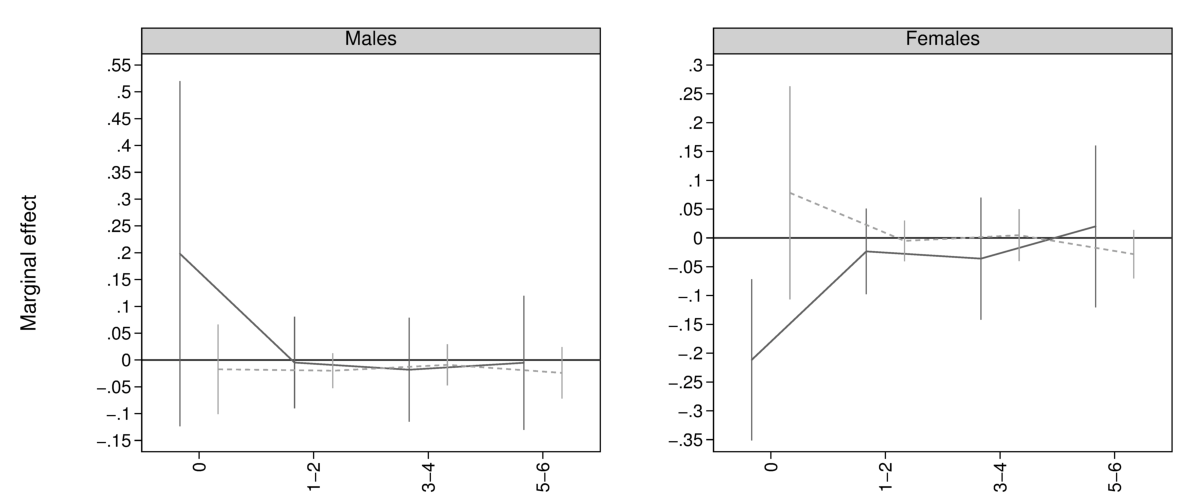
\includegraphics[width=\linewidth]{Chapter5/Figures/mi_msm_l_all_obese.pdf}
Fixed effects
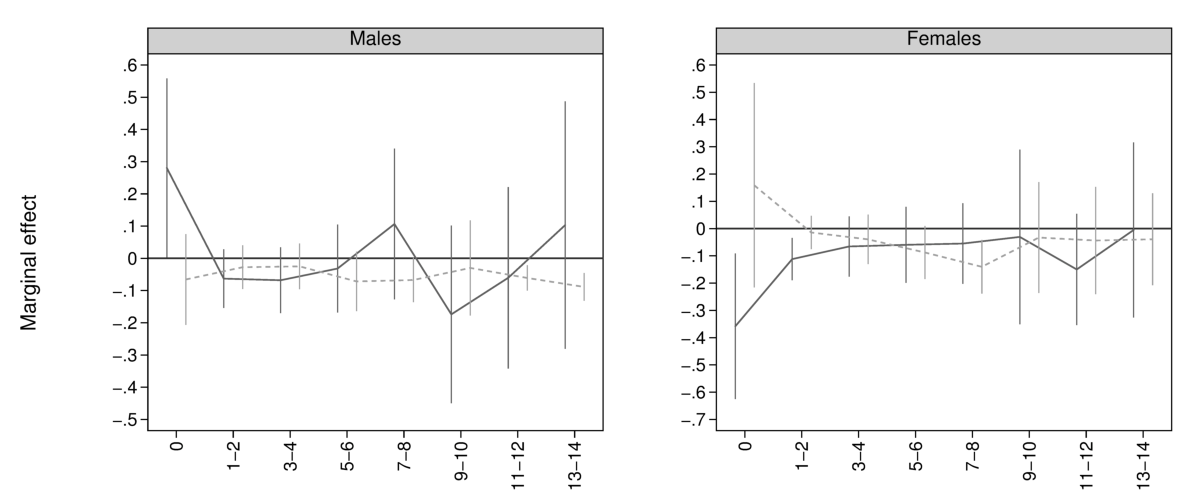
\includegraphics[width=\linewidth]{Chapter5/Figures/mi_obese_fe.pdf}
Random effects
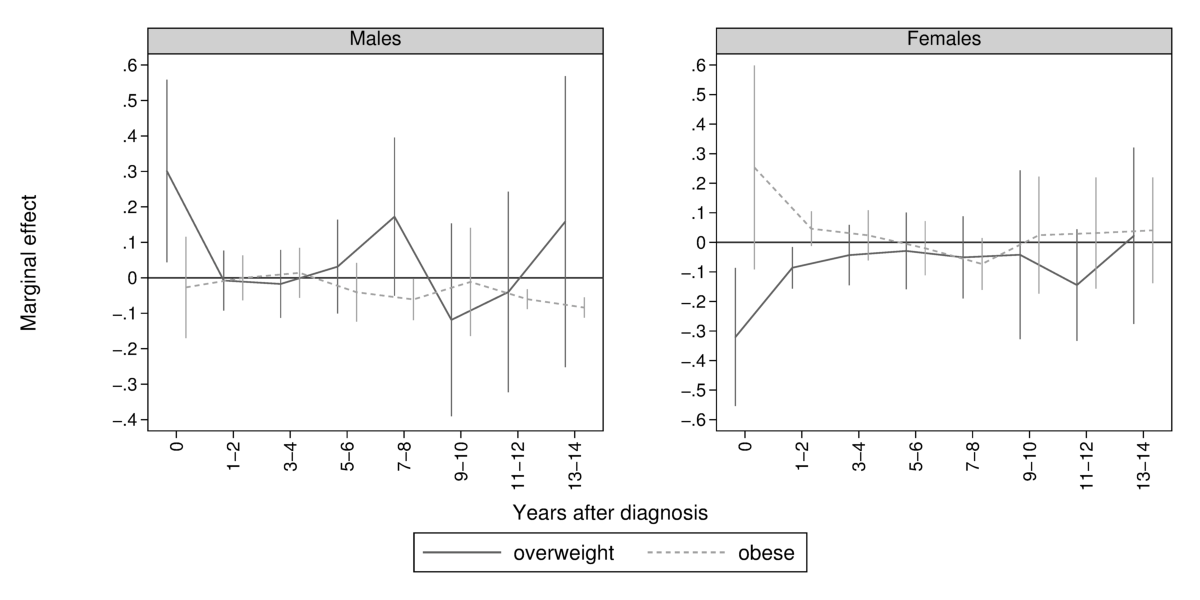
\includegraphics[width=\linewidth]{Chapter5/Figures/mi_obese_re.pdf}
\footnotetext{\textit{Notes} 95\% confidence intervals}
\end{center}
\end{figure}
\clearpage